\documentclass[12pt,twoside]{report}
%load packages
\usepackage[utf8]{inputenc}
\DeclareUnicodeCharacter{2009}{\,} 
\usepackage[english]{babel}
\usepackage{csquotes}
\usepackage[a4paper,width=150mm,bindingoffset=6mm,top=25mm,bottom=25mm,headheight=15pt]{geometry}
\usepackage{graphicx}
\usepackage{float}
\graphicspath{{/home/ericulrich/Documents/Master/Masterarbeit/LaTeX_thesis/Main/Images/}{/home/ericulrich/Documents/Master/Masterarbeit/LaTeX_thesis/Introduction/Images/}{/home/ericulrich/Documents/Master/Masterarbeit/LaTeX_thesis/Materialsandmethods/Images/}{/home/ericulrich/Documents/Master/Masterarbeit/LaTeX_thesis/Results/Images/}{/home/ericulrich/Documents/Master/Masterarbeit/LaTeX_thesis/Materialsandmethods/Images/}{/home/ericulrich/Documents/Master/Masterarbeit/LaTeX_thesis/Supplementary/Images/}}
\usepackage{amsmath}
\usepackage{refcheck}
\usepackage{textgreek}
\usepackage{hyperref}
\usepackage{gensymb}
\usepackage{lmodern,textcomp}
\usepackage{color, colortbl}
\definecolor{LightCyan}{rgb}{0.88,1,1}
\usepackage{texshade}
\usepackage{longtable}
\usepackage{dnaseq}
\usepackage{tabularx}
\usepackage{pdfpages}
\usepackage{multirow}
	\newcolumntype{L}{>{\raggedright\arraybackslash}X}
\usepackage[table,xcdraw]{xcolor}
\usepackage{dirtytalk}


\bibliographystyle{unsrt}

\usepackage{fancyhdr}
\pagestyle{fancy}
\fancyhead{}
\fancyhead[LO,LE]{\leftmark}
%\fancyhead[RO,RE]{\rightmark}
\fancyfoot{}
\fancyfoot[LO,LE]{Eric Ulrich}
\fancyfoot[CO,CE]{\thepage}
\fancyfoot[RO,RE]{University of Basel}




\usepackage[backend=biber,sorting=none,style=numeric,citestyle=numeric]{biblatex}
\usepackage{url}
\setcounter{biburllcpenalty}{7000}
\setcounter{biburlucpenalty}{8000}
\addbibresource{/home/ericulrich/Documents/Master/Masterarbeit/LaTeX_thesis/Main/bibliography.bib}
\begin{document}

\begin{titlepage}
	\begin{center}
		\includegraphics[width=0.4\textwidth]{logo}\\
		\vspace{1cm}
		\Large
		Faculty of Science \\
		Department Biozentrum\\
		University of Basel\\
		Switzerland\\
		\date{\today}
		\vspace*{1cm}
		
		\Huge
		Master thesis Molecular Biology \\
		\vspace{2cm}
		\LARGE
		\textbf{Studying cefepime resistance evolution in ESBL \textit{Escherichia Coli} patient isolates and experimentally evolved ESBL \textit{Escherichia Coli} strains}
		
		\vspace{3cm}
		\begin{minipage}[t]{0.47\textwidth}
			\textnormal{\large{\bf Submitted to:\\}}
			{\large Prof. Dr. Richard Neher\\ Prof. Dr. Dirk Bumann}
		\end{minipage}\hfill\begin{minipage}[t]{0.47\textwidth}\raggedleft
			\textnormal{\large{\bf Submitted by:\\}}
			{\large Eric Ulirch}
		\end{minipage}			
		\vspace{3.5cm}
		\newline 
		\large{\today}

		
		
	\end{center}
\end{titlepage}
\pagenumbering{roman}
\chapter*{Abstract}
\addcontentsline{toc}{chapter}{Abstract}
In Swiss hospitals infections with extended-spectrum cephalosporin resistant \textit{Escherichia coli} (\textit{E. coli}) are emerging \cite{swiss_hospitals}. Enzymes called extended-spectrum \textbeta-lactamases (ESBL) are able to hydrolyze extended-cephalosporins. If expressed in \textit{E. coli}, the susceptibility to extended-cephalosporins is reduced and the strains are called ESBL \textit{E. coli}. Research  heavily focused on studying ESBL mediated extended-spectrum cephalosporin resistance, even though other resistance mechanisms possibly affect extended-spectrum resistance level. We studied cefepime resistance evolution in order to possibly identify new genotypes associated with drug resistance. Therefore, we studied whole-genome sequencing data from ESBL \textit{E. coil} isolates from patients of the University Hospital of Basel evolving resistance to cefepime in patients. Additionally, we assembled a device called morbidostat which we used to experimentally evolve resistance to cefepime with ESBL \textit{E. coli} strains. The morbidostat is an automated culturing device continuously applying high antibiotic pressure to cultures resulting in resistance evolution. We cultured three ESBL \textit{E. coli} strains with the morbidostat which increased the minimal inhibitory concentration of cefepime tested with the strains after culturing with the morbidostat over 100 fold. We analyzed whole-genome sequencing data of the strains cultured with the morbidostat and identified several single nucleotide polymorphisms (SNPs). Interestingly we found SNPs targeting the same gene in patient isolates and morbidostat samples, strongly suggesting the importance of the SNP for the resistance. In particular we identified SNPs in patient isolates and morbidostat samples targeting the genes coding for the porins \textit{ompC} and \textit{ompF} and their regulatory system. Furthermore, SNPs affected the transcription unit by targeting the genes coding for the DNA-directed RNA polymerase subunit \textbeta \space and the RNA polymerase sigma factor.  
\chapter*{Acknowledgments}
\addcontentsline{toc}{chapter}{Acknowledgments}
I would like to thank my group leader Richard Neher who made this very interesting project possible. 
\tableofcontents
\pagenumbering{arabic}
\chapter{Introduction}

\section{Cause and urgency of antibiotic resistance}
The discovery of Penicillin shortly before the Second World War has revolutionized human medicine in the western world by saving the lives of millions of soldiers and civilians. It also made major advances in surgery possible. Ever since then antibiotics play a very important role in our well established health system and we are depending on those drugs in order to fight bacterial infections \cite{worldwar_resistance}.

Because of the positive experience people made during the Second World War with antibiotics, they quickly started to use them in an irresponsible way. This caused a Penicillin resistance within 32 years after it's discovery \cite{worldwar_resistance}. Therefore people realized early on, that extensive use of antibiotics are a thread for the efficiency of those drugs. But the discovery of new antibiotics gave them confidence and the excess of usage of antibiotics went on. Not only were antibiotics continuously prescribed inappropriately they also got introduced into agriculture.
Unfortunately the tendency of irresponsible use of antibiotics increased in the last couple decades. 

For Switzerland the rate of antibiotic consumption divided by the Swiss population stayed the same in recent times, but the absolute consumption increased. This is because more people were getting treated in hospitals \cite{swiss_hospitals} but the general population of Switzerland increased too.     
Furthermore antibiotic resistance is a global issue. Compared to other countries Switzerland is on the lower end when it comes to antibiotic doses per 1000 people \cite{swiss_hospitals}. Additionally other countries also have a very high use of antibiotics in agriculture, exposing a lot of bacteria to a lot of antibiotics, giving the bacteria an ideal environment to evolve and gains resistance. Since traveling started to get a lot more popular with long-distance traveling in particular, there is a globally ongoing exchange of resistant pathogens. This increases the difficulties of managing resistant pathogens because fighting the antibiotic resistance crisis locally is not going to help much because of this global exchange.  

In Switzerland the biggest challenge with resistant pathogens is ongnoind in hospitals. In such institutions, obviously a lot of people need treatment against bacterial infections, leading to an accumulation of pathogens but also to very locally applied high doses of antibiotics.
Therefor Swiss hospitals turned into hot-spots of antibiotic resistant pathogens.
Unfortunately a lot of people within the hospitals are weakened by diseases causing a worse functional immune system and therefore such patients are a lot more vulnerable to infections with antibiotic resistant bacteria.
This combination of an increasingly number of antibiotic resistant bacteria and very vulnerable patients lead to a very urgent problem in modern medicine causing about 300 deaths, patients having to spend more time in hospitals and high costs \cite{anresis}.

\subsection{An overview of antibiotic resistant pathogens in Swiss hospitals}
Mainly four strains which cause problems in treatment with antibiotics are present in Swiss hospitals:\\
\begin{figure}[H]
	\includegraphics[scale=0.2]{pathogens_overview.png}
	\caption{Development of popularity of antibiotic resistant pathogens.
	\cite{swiss_hospitals_pathogens}}
	\label{figure:pathogen_dvelopment}
\end{figure}
\textbf{Staphylococcus aureus} usually doesn't cause any diseases in healthy people. But if someone's immune system is weakened they can cause skin and bone inflammations. Staphylococcus aureus is causing the most infections for surgical wounds.

\textbf{Streptococcus pneumoniae} are present normally in the nose and throat of everyone. For weak people this strain can turn into a pathogen causing several thousands blood infections and pulmonary infections per year. 

\textbf{Klebsiella pneumoniae} is one of the biggest problems for swiss hospitals. They can cause severe pulomnary infections and blood infections which can be very dangerous for newborns \cite{swiss_hospitals_pathogens}.

\textbf{Escherichia coli (E. coli)} belongs to the enterobacteriaceae and is present in every intestine where they are not dangerous. However they are able to cause infections when present in other parts of the body leading mainly to infections of the urinary tract but also in the brain of new borns. 

Mainly E. coli and Staphylococcus aurei have been increasingly reported in context of antibiotic resistant infections over the last 15 years as visible in Figer \ref{figure:pathogen_dvelopment}. On the other hand antibiotic resistant infections with Streptococci pneumoniase and Entereococcus remained more or less the same or decreased slightly.
It is noteworthy how fast the numbers of infections with extended spectrum \textbeta-lactamase (ESBL) producing E. coli increased within 15 years. In 2004 they only made up for about 1 \% of all antibiotic resistant pathogens, 2018 they are already at 12 \% with an uprising tendency. This is causing a lot of concerns and problems in hospitals because as the name already implies, those pathogens are able to hydrolyze an extended spectrum of \textbeta-lactams forcing doctors to prescribe antibiotics of last resort.

Because of this threat coming from ESBL E. coli I dedicate this thesis entirely to this pathogen. Unfortunately it is not completely understood yet, how those enterobacteriaceae are able to produce such a strong resistance against many \textbeta-lactams. My goal is to generally get a better understanding of genes involved in the evolution of resistance and potentially identify new genes which could play an important role in the resistant mechanisms. 

\section{Extended-spectrum -lactamases (ESBL) E. Coli}
Extended \textbeta-lactamases (ESBLs) are certain \textbeta-lactamases which are able to hydrolyze extended-spectrum cephalosporins with an oxyimino side chain. Such cephalosporins are aztronam, cefotxamie or ceftazidime for example \cite{esbl_introduction}. 
Some ESBLs arose by mutations in genes for common plasmid-mediated \textbeta-lactamases such as TEM and SHV enyzmes. Those ancestors were able to hydrolyze regular \textbeta-lactamases but were susceptible to cephalosporins \cite{esbl_introduction_emerg}. 
There are also new families of ESBLs, such as CTX-M and OXA \cite{ctx-m} which evolved independently from the ESBLs which have their origin in the TEM and SHV enzymes. 

Those newly formed \textbeta-lactamases are increasingly reported as reasons for resistance, in contrast to the other \textbeta-lactamases related to TEM and SHV which generally decrease in popularity.
CTX-M is a group of \textbeta-lactamases with CTX-M-1 being the most popular one. There are many more characterized CTX-M enzymes, most of them differ by just one amino acid. With a sequence identity compared to TEM and SHV of only 40 \% \cite{ctx-m}, it's assumed that they evolved from a different precursor. It's assumend that they evolved from the \textbeta-lactamase precursor AmpC from Klyzvera ascorbata  \cite{ctx-m}. Even though the first CTX-M-1 was isolated in Germany, it's mostly popular in eastern Europe, South America and Japan.
The OXA family was originally created as a phenotypic rather than a genotypic group, based on a specific hydrolysis profile. Therefor the sequence identity compared to other members of this family is only about 20 \%. It's name comes from the ability to efficiently hydrolyze oxacillin \cite{ctx-m}.
   
ESBL E. Coli can be detected using isothermal amplification, PCR or microarrays. Since ESBL E. coli are able to hydrolyze cephalosporine, doctors prescribed carbapenems or potent \textbeta-lactam-\textbeta-lcatamase inhibitor (BLBLI) combinations, when ESBLs were detected with the methods above. However it turned out that some E. coli expressing ESBLs are actually susceptible to oxymino-cephalosporins \cite{esbl_introduction}. This showed, that the prescription of antibiotics of last resort because a pathogen tested positive for ESBLs was unnecessary in some cases. Since antibiotics of last resorts are incredibly valuable it's in the interest of everyone to only use them if urgently necessary. Irresponsible prescription on the other hand will cause further resistance in a rather short time scale. 
Since a simple presence/absence check of ESBLs is not giving the necessary information in order to decide whether antibiotics of last resort are needed, those tests are now getting ignored as ordered by the EUCAST \cite{eucast}. It's recommended to test susceptibility in vitro which takes about 48 hours which is a lot longer than genetically testing. For patients in acute stages of inflammation 48 hours is too long, forcing doctors to still prescribe antibiotics of last resort even when it's not known if the pathogen would be susceptible to common cephalosporins. 
Since some ESBL producing E. coli are genetically resistant but phenotypically susceptible there must be other mechanisms involved in the resistance path next to a simple presence or absence of \textbeta-lactamases. 

Other ways to protect the pathogen from the drug could be a less permeable outer membrane of the pathogen. It's also possible that resistant pathogens have a higher efflux activity, leading to an active transport of the drug, out of the cell. In combination this would mean a lower influx and a higher efflux, which would work in favor of the pathogen. Furthermore another option would be that the copy number of genes coding for ESBLs varies within ESBL E. coli, deciding over resistance or susceptibility. 

With this thesis I try to get a better understanding on which strategies are involved in resistant ESBL E. coli. I'm doing this by combining two different approaches, one being a bioinformatic analysis with ESBL E. coli isolates from patients, the other being a more experimental approach.\\ 


For the first part of this project I try to identify changes in the genome from ESBL E. coli samples isolated from our collaborator Adrian Egli at the University hospital Basel. Those samples made a transformation from being susceptible to \textbeta-lactams to resistant, or they lost their ability to hydrolyze cephalosporins. 

For the experimental part of this project I assemble a system called morbidostat which allows to continuously monitor E. coli cultures and automatically putting them under antibiotic pressure, by injecting appropriate drug doses. This causes evolution and selection which can be observed in real time. Along this process samples can be taken and analyzed with a similar pipeline as for the clinical isolates.

\section{Longitudinally collected ESBL E. coli isolates from patients from the University hospital Basel}
Our collaborator Adrian Egli, head of the clinical microbiology from the University hospital Basel, collected Isolates of patients who were infected with ESBL E. coli. His group determined the MIC of the cephalosporines cefepime and ceftazidime for every collected isolate  and short-read sequenced thme on a MiSeq Illumina system.
This resulted in a data collection with multiple isolates per patient, where a change of MIC for cefepime and ceftazidime was visibile over time caused by gained or lost resistance. 
The principle of this analysis is, to build a very accurate reference genome for each patient based on the isolate with the lowest MIC for the tested cephalosporines. The isolate with the lowest MIC is also called wild-type. Then the other isolates with a higher MIC can be compared to this reference genome and changes can be identified. 

This can be done by mapping the Illumina sequencing data from the resistant isolates to the reference genome from the wild-type. 
This makes possible to identify single-nucleotide polymorph positions (SNPs) in the genome of the resistant samples. Because tools for annotating genomes are available, it's possible to filter for SNPs which are affecting known genes or promoter regions. Based on this information it should be possible to get more insights in the evolution of resistance. 

Since this analysis is depending on very accurately assembled reference genomes we additionally long-read sequenced isolates of interest with Oxford Nanopore Technologies. Illumina returns very accurate short reads (75 bp) but because the reads are so short it's computationally not possible to assemble those reads structurally correct. On the other hand reads produced with Nanopore Technologies are extremely long (up to 200 kbp) but quite inaccurate based on issues with repetitive nucleotide sequences. However both techniques combined together return an assembly with a nucleotide error rate from Illumina but also with a high accuracy in terms of structural information.  
This strategy of combining short- and long-reads is also known as hybrid assembly. 


\section{Building a morbidostat} 
Since we wanted to experimentally force susceptible ESBL E. coli to gain resistance over a rather short time period, we had to come up with a system which allows to constantly put E. coli under antibiotic pressure. Such constant antibiotic pressure forces evolution of resistance and for selection of mutants. Such a system has already been invented by Toprak et al. \cite{morb_toprak} which he called morbidostat, an automated continuous culture device. Based on the invention of Toprak we rebuild a morbidostat with small modifications which should improve the handling and mainly make it a lot more compact which is important since we want to use the morbidostat in a space limiting hypoxi-station. With our version of the morbidostat 15 cultures can be grown independently in vials. Thereby the growth of each culture is monitored by measuring and saving the optical density (OD). Based on the growth an appropriate dose of antibiotics is injected into the culture leading to an inhibition of the growth without entirely killing ever colony forming unit. The appropriate dose of antibiotics is achieved by mixing different drug concentrations using computer controllable pumps which are also injecting the drug into the vials.
The morbidostat allows to study drug resistance evolution in real-time, while having an idea of the progress of evolution in resistance. Since the goal is to identify changes in the genome while the strain gains resistance, samples have to be collected every other day, in order that the DNA can be isolated and sequenced.

In the morbidostat, bacteria are grown in a fixed volume. The process of suppressing the growth with antibiotics is divided into cycles which are constantly getting executed. One cycle has following tasks and commands:
\begin{itemize}
	\item Measuring the OD every several seconds over a defined cycle time \textDelta t 
	\item Calculating growth rate at the end of the cycle based on the previously collected ODs
	\item Based on growth, injection of appropriate dose of drug, as calculated by a feedback algorithm
	\item Getting rid off volume which exceeds fixed culture volume
\end{itemize}

\begin{figure}
	\includegraphics[scale=0.1]{vial_diagram.png}
	\includegraphics[scale=0.07]{growth_diagram.png}
	\caption{Based on the growth a feedback algorithm decides whether and how much drug is getting injected}
	\label{figure:vial_setup}
\end{figure}

\subsection{Drugs of interest and bacteria of choice for the experiments}
\subsubsection{Choice of ESBL bacteria for the morbidostat experiments}
Initially the idea was to cultivate the wild-type isolates from the sample collection provided from Adrian Egli and which were also used for the bioinformatics analysis. This would have been nice, because it would have allowed to compare evolution taking place under physiological conditions and forced evolution by the morbidostat. 
Even though the morbidostat is run inside an air tight hypoxystation within a bio safety lab 2, it was decided that it's to risky to do the experiments with the ESBL E. coli coming from the hospital. Instead we decided to clone the \textbeta-lactamase sequences from the wild type samples into a plasmid transformed into K12 E. coli which is not able to infect humans.

Concerning the drugs, cefepime and cefatzidime were chosen, since those drugs were also used for the treatment of the ESBL E. coli from the sample collection from the hospital.\\
Both caphalosporines are effectively bactrocidal against gram-negative bacteria and act by inhibiting the synthesis of the peptidogylcan layer of gram negative bacterial cell walls. cefepime is reagrded as a 4th-generation cephalosporin and was developed with ceftazidime as a foundation. Reistance against ceftazidime often emerged due to hydrolysis by the AmpC \textbeta-lactamase. Cefepime was designed with a change in its 3' side chain, which should protect the drug from hydrolysis \cite{cefepime}.  








 








\chapter{Materials and methods}
This chapter summarizes the material and methods used in this work. ESBL \textit{E. coli} isolates which gained resistance to cefepime and ceftazidime in patients of the University Hospital of Basel were analyzed with a bioinformatic pipeline. Furthermore a morbidostat was assembled which we used to experimentally evolve resistance to cefepime with ESBL \textit{E. coli}. SNPs as a product of resistance evolution were identified following the same bioinformatic pipeline as for the isolates obtained from patients. Code written for running the morbidostat or for identifiyng SNPs is available on  https://github.com/nahanoo/ESBL\_project.

\section{ESBL \textit{E. coli} isolates from patients at the University Hospital of Basel}
Our collaborators from the clinical microbiology of the University Hospital of Basel provided an isolate collection of 65 ESBL \textit{E. coli} isolates sampled from 34 patients resulting in multiple isolates per patient. Isolates from the same patient are referred to as an isolate series. They determined the isolates as ESBL producing by carrying out combination disk diffusion tests. Furthermore, they determined the minimal inhibitory concentration (MIC) of cefepime and ceftazidime for every isolate. We selected isolate series, where the susceptibility of the isolates changed over the sampling period and where phylogenetic analysis ensured, that every isolate of a series was the same strain. Of every selected isolate series we identified SNPs which were potentially caused by resistance evolution. 
\label{section:sample_collection}

\subsection{Disk diffusion tests}
As recommended by the EUCAST the research group of Adrian Egli from the clinical microbiology at the University Hospital of Basel determined the \textit{E. coli} isolates as ESBL producing by carrying out standardized disk diffusion tests. \\
They prepared a cell suspension of each isolate equal to 0.5 McFarland standard. Those suspensions were spread over the entire area of Mueller Hinton agar plates. On those plates disks with ether 30 \textmu g ceftazidime, 30 \textmu g ceftazidime + 10 \textmu g clavulanic acid, 30 \textmu g cefepime and 30 \textmu g cefepime + 10 \textmu g clavulanic acid were applied. All plates were incubated for 20 hours. The inhibition zones caused by the disks were measured, if the inhibition diameters were larger than 5 mm the isolates were deterimed as ESBL producing. All of the isolates form the collection turned out to be ESBL producing. 

\subsection{MIC determination}
The MICs of every isolate were determined by the research group of Adrian Egli for the antibiotics ceftazidime and cefepime. This allowed us to select patients with isolates changing their susceptibility over time. \\
The MICs were determined by performing E tests. From an agar plate they picked a few colonies and diluted the, to 0.5 McFarland with physiological NaCl-solution. The suspension was plated on an agar plate. A reagent strip with either a ceftazidime or cefepime gradient was placed in the middle of the plate. After 20 hours the resulting minimal inhibitory concentration (MIC) was checked.

\subsection{Selection of isolates suitable for our analysis}
We only analyzed isolate series which consisted of more than one isoalte, showed a significant change of the MICs and were all the same ESBL \textit{E. coli} strain. To ensure that a isolate series consisted of the same strain, we performed a phylogenetic analysis with every isolate. This analysis was based on Illumina sequences of the isolates provided by our collaborator. For the phylogenetic analysis we used a tool called PanX \cite{ding_panx:_2018}.

\subsubsection{Illumina sequencing}
The DNA from the isolates was extracted using the EZ1 DNA tissue kit on an EZ1 Advanced XL robotic system (Qiagen). The library for the sequencing was prepared using the Nextera XT library preparation kit (Illumina) and the resulting library was sequenced on a MiSeq Illumina platform \cite{nanopore}. The reads produced with Illumina were trimmed with Trim Galore \cite{noauthor_babraham_nodate}.
\label{section:illumina}

\subsubsection{PanX}
PanX is a tool which clusters genes into orthologous clusters \cite{panx}. From those clusters, panX identifies the core genome which are genes shared by all isolates in the cluster. Based on those core genomes a strain-level phylogeny is built, making use of single nucleotide polymorph positions (SNPs) within the core genomes \cite{panX}. This resulted in a phylogenetic tree with the information how closely related the isolates were. \\ 
PanX uses annotated whole-genomes as input files, this is why every isolate was short-read assembled and annotated. For short-read assembling we used spades and for annotating the resulting assemblies we used prokka \cite{nurk_assembling_2013} \cite{seemann_prokka:_2014}. Prokka first searches a core set of well characterized proteins using BLAST+ and then compares reading frames to a database derived from UniProtKB \cite{seemann_:zap:_2019}. The results from prokka were stored in a genbank file for every isolate. The PanX analysis was performed, based on those genbank files. \\

\subsection{Identification of SNPs}
Considering the phylogenetic analysis and the MICs we selected five patients with at least two isolates per patient which we analysed. Because the pipeline for identifying SNPs was based on Illumina ONT sequencing data, we sequenced every selected isolate with ONT. 
Afterwards the selected isolate series were analyzed with the pipeline described in Section \ref{section:pipeline}.
\subsubsection{ONT sequencing}
For ONT sequencing the library with the isolates was prepared with a ligation sequencing kit (LSK-108) followed by the native barcoding expansion kit. This allowed barcoding of multiple isolates and loading all of them on a single flow cell (FLO-MIN106D). As a sequencing device we used the MinION from ONT. \\
As a fist step each DNA isolate was diluted to a concentration of 20 ng/\textmu L in 50 \textmu L nuclease free water (NFW). For end-repairing the DNA 7 \textmu L NEBnext Ultra II Endrepair/dA-tailing enzyme mix was added to each
isolate and incubated at 20\degree C for 5 min and at 65\degree C for 5 min. After this step every isolate was cleaned up by adding 60 \textmu L of AMPure XP beads. The beads were incubated with the isolates for 5 minutes on a rotator and then removed on a magnetic rack. Every isolate was washed with 200 \textmu L 70\% ethanol which was repeated once. The ethanol was removed and every isolate was suspended in 25 \textmu L NFW. 2.5 \textmu L of each barcode plus 25 \textmu L of Blunt/TA ligase was added to each isolate and incubated for 10 minutes. All the isolates were pooled and 500 \textmu L of AMPure XP beads were added. After incubating the pooled isolate for 5 minutes on the rotator the isolate was washed again twice with 70 \% ethanol. All the DNA was eluted in 51 \textmu L NFW. The final isolate was diluted to a concentration of 35 ng/\textmu L. Then for adapter ligation 20 \textmu L BAM, 30 \textmu L Ultra II ligation master mix and 1 \textmu L enhancer were added. After 10 minutes of incubation, 40 \textmu L AMpure XP beads were added and incubated on the rotator for 5 minutes. The supernatant was removed on the magnetic rack and the DNA was washed twice with ABB. The DNA was eluted and incubated for 10 minutes in 15 \textmu L ELB. Finally the library was prepared by mixing 15 \textmu L of eluted DNA in ELB with 25.5 \textmu L LLB and 35 \textmu L RBF. The resulting library was loaded on the flow cell, which was primed before with a mixture of 480 \textmu L RBF  and 520 \textmu L of NFW. The sequencing run was started and simultaneously base-called with Albacore.
\label{section:nanopore_sequenicng}

\subsection{Studying copy numbers of ESBL genes}
We were also interested to see if the copy numbers of ESBL genes changed while resistance evolved. Possibly the copy numbers affect the ESBL protein level which could explain extended resistance. Therefore, we hybrid-assembled every selected isolate with Unicycler \cite{wick_unicycler:_2017} and annotated the assembly with prokka \cite{seemann_prokka:_2014}. Afterwards we checked how many ESBL genes were present considering the annotation provided by prokka.

\section{Bioinformatic pipeline for identifying SNPs accumulated by evolving resistance against cefepime in ESBL \textit{E. coli}}
\label{section:pipeline}
\begin{figure}
	\includegraphics[width=0.9\textwidth]{pipeline.png}
	\caption{Bioinformatic pipeline used for the identification of mutations and affected genes/promoters.}
	\label{figure:pipeline}
\end{figure}
The foloowing pipeline was used to identify SNPs in isolate series which evolved resistance. This pipeline was based on Illumina and ONT sequencing data coming from multiple isolates which were taken while resistance evolved. In principle a hybrid-assembly of the genome was performed for the isolate with the lowest MIC. This genome was used as a reference in order to identify SNPs accumulated in the other isolates where resistance evolved. We also tried to provide annotation for the SNPs. 

\subsection{Creating a reference genome with annotation} 
As a first step we hybrid-assemblied the genome of the isolate with the lowest cefepime MIC of an isolate series with Unicycler \cite{wick_unicycler:_2017}. Every assembly was annotated with prokka which produced a genbank file for every reference genome \cite{seemann_prokka:_2014}. Additionally promoter regions were identified using the promoter prediction tool PePPER \cite{pepper}. PePPER is a tool which takes whole-genomes as an input and predicts promoter sequences. Those sequences were mapped against the reference genome using graphmap \cite{sovic_fast_2016}. Furthermore, a promoter data base hosted on EcoCyc was used. This database contains around 3800 experimentally validated promoters for \textit{E. coli}\cite{noauthor_smarttable_nodate}. The sequences from this database were downloaded and mapped against the reference genome with graphmap as well \cite{sovic_fast_2016}. 
\label{section:annotatiion_ref}.

\subsection{Mapping Illumina sequencing data of the isolate series to the reference genome}
As a second step of the pipeline the short-read Illumina sequencing data of every isolate was mapped against the reference genome of the isolate series. Mapping to the reference genome was done with BWE mem \cite{li_fast_2009}. This resulted in a bam file for every isolate of the series. Mapping all the Illumina reads provided us the information which base was present in every Illumina read mapped to a certain position to the reference genome. If the most abundant base of all Illumina reads at a certain position is different than in the reference genome a SNP was present. To make this information more accessible we calculated pile-ups as a third step of our analysis. 

\subsection{Calculating pile-ups}
Pile-ups are count matrices storing which base is present how many times at a certain position considering every mapped Illumina read. In order to produce those pile-ups we used a script called \href{https://github.com/nahanoo/ESBL\_project/pileup.py}{pileup.py}. This script extracted the base counts by going through every position of the sorted bam-file from an isolate. Pile-ups were calculated for every isolate of a series and all the pile-ups stored in a matrix stack.

\subsection{Identification of SNPs} 
We identified SNPs by comparing the most abundant base at every position of the matrix-stack with a script called \href{https://github.com/nahanoo/ESBL\_project/pileup.py}{analysis\_modular.py}. If the most abundant base varied between the isolate a SNP was identified. For the rest of the pipeline only SNPs were included where the coverage was at least 30 and the base frequency at least 0.8.

\subsection{Identifying genes and promoters affected by mutations}
As a last step of the pipeline we checked if annotation was available for the SNPs. For checking if a SNP affected a gene, we analyzed the genbank file with biopython \cite{cock_biopython:_2009}. To check whether a SNP affected a promoter region we analyzed the bam-files which were created with the promoter sequences from PePPER and EcoCyc. We checked if a SNP was located between a start or end position of a mapped promoter sequence. 

\section{Assembling the morbidostat}
We experimentally evolved resistance to cefepime with ESBL \textit{E. coli} strains using a morbidostat. We assembled an adapted version of Topraks built differing mainly in its pump system, controlling unit and software\cite{toprak_building_2013}. Hardware which was not commercially available was built by the in-house mechanic and electronic workshop.

\begin{figure}
	\includegraphics[width=0.7\textwidth]{setup_annotated_inksacpe.png}
	\includegraphics[width=0.4\textwidth,angle=90]{vial.JPG}
	\caption{Left: Overview of the morbidostat setup. Vials were placed on magnetic stirrer and connected to three drug injecting pumps and one waste removal pump. A microcontroller was connected in serial to a PC, which allows to computer control drug injections and OD measurements. Right: One vial with all the inlets.}
	\label{figure:morbidostat_setup}
\end{figure}  
Figure \ref{figure:morbidostat_setup} shows the morbidostat setup.
As a base for our build we used a magnetic stirrer with 15 slots. On that stirrer we placed three layers of acrylic glass through which we inserted black plastic rings which acted as our vial holders and optical density (OD) measuring units. 
The vials placed in the vial holders had three inlets as shown in Figure \ref{figure:morbidostat_setup}. One inlet was used to inject media or antibiotics, one for removing volume exceeding the culture volume and the last one to mount an air filter for pressure equilibration. \\
To test the hardware, we built the morbidostat in the open as shown in Figure \ref{figure:morbidostat_setup}. For the actual experiments we placed the morbidostat inside a hypoxi-station in a bio safety lab 2. This allowed us to culture the bacteria at 37 \degree C but also to increase the safety. 


\subsection{OD measuring units}
For measuring the ODs we sent a ray of light through the cultures. This ray was scattered by the cells meaning that the ray was thrown off by the cells in multiple directions. With the help of a phototransistor we could measure the scattering with analog pins of the microcontroller. Because the scattering was proportional to the cell density, we could translate the scattering into an OD by calibration. \\
One OD measuring unit integrated in the vial holder is shown in Figure \ref{figure:OD_unit}. Every unit consisted of a vertical-cavity surface-emitting laser (VCSEL) and a phototransistor. We chose OPB608V as a VCSEL with a peak wavelength of 890 nm and PT 333-3C as a phototransistor, both from TT electronics. For each unit the VCSEL and the phototransistor were placed in a 135 \degree \space angle inside the vial holder. Both components were in direct contact with the glass vial.
The 15 OD measuring units were divided into three groups of five units which corresponds to one row of vials of the morbidostat. For every group the VCSELs and phototransistors were both connected to independent 5 V circuits. The circuits of one group are illustrated in the left Figure \ref{figure:OD_cirguit}, where the VCSEL circuit is shown orange and the phototransistor circuit in blue. \\
The VCSELs were constantly on sending rays of light through the cultures. When an OD measurement was initialized the scattering was detected with the phototransistors. Light reaching the phototransistor caused an opening in the semiconductor from the phototransistor which led to an amplification of the current. This current reached a potentiometer connected in serial over which we measured the voltage with an analog pin of the microcontroller. The opening of the semiconductor altering the measured voltage correlated with how much light reached it. More cells caused more scattering and more light reaching the semiconductor. Therefore, there was a linear correlation between the measured voltage and the cell density in the suspension. \\

\label{section:OD}
\begin{figure}
	\includegraphics[width=0.6\textwidth]{OD_setup.png}
	\includegraphics[width=0.3\textwidth]{OD_unit.png}
	\caption{Left: Circuit for parallel connected VCSELs (orange). Each VCSEL is connected in serial with a 220 \textOmega \space resistor. The circuit of the phototransistors is shown in blue. The phototransistors are connected in parallel. Each phototransistor is connected to a potentiometer in serial over which the voltage is measured with an analog pin of the microcontroller.}
	\label{figure:OD_cirguit}
	\label{figure:OD_unit}
\end{figure}

\subsection{Pumps and tubing} 
\begin{figure}
	\includegraphics[width=0.2\textwidth]{piezo.png}
	\includegraphics[width=0.4\textwidth]{board.JPG}
	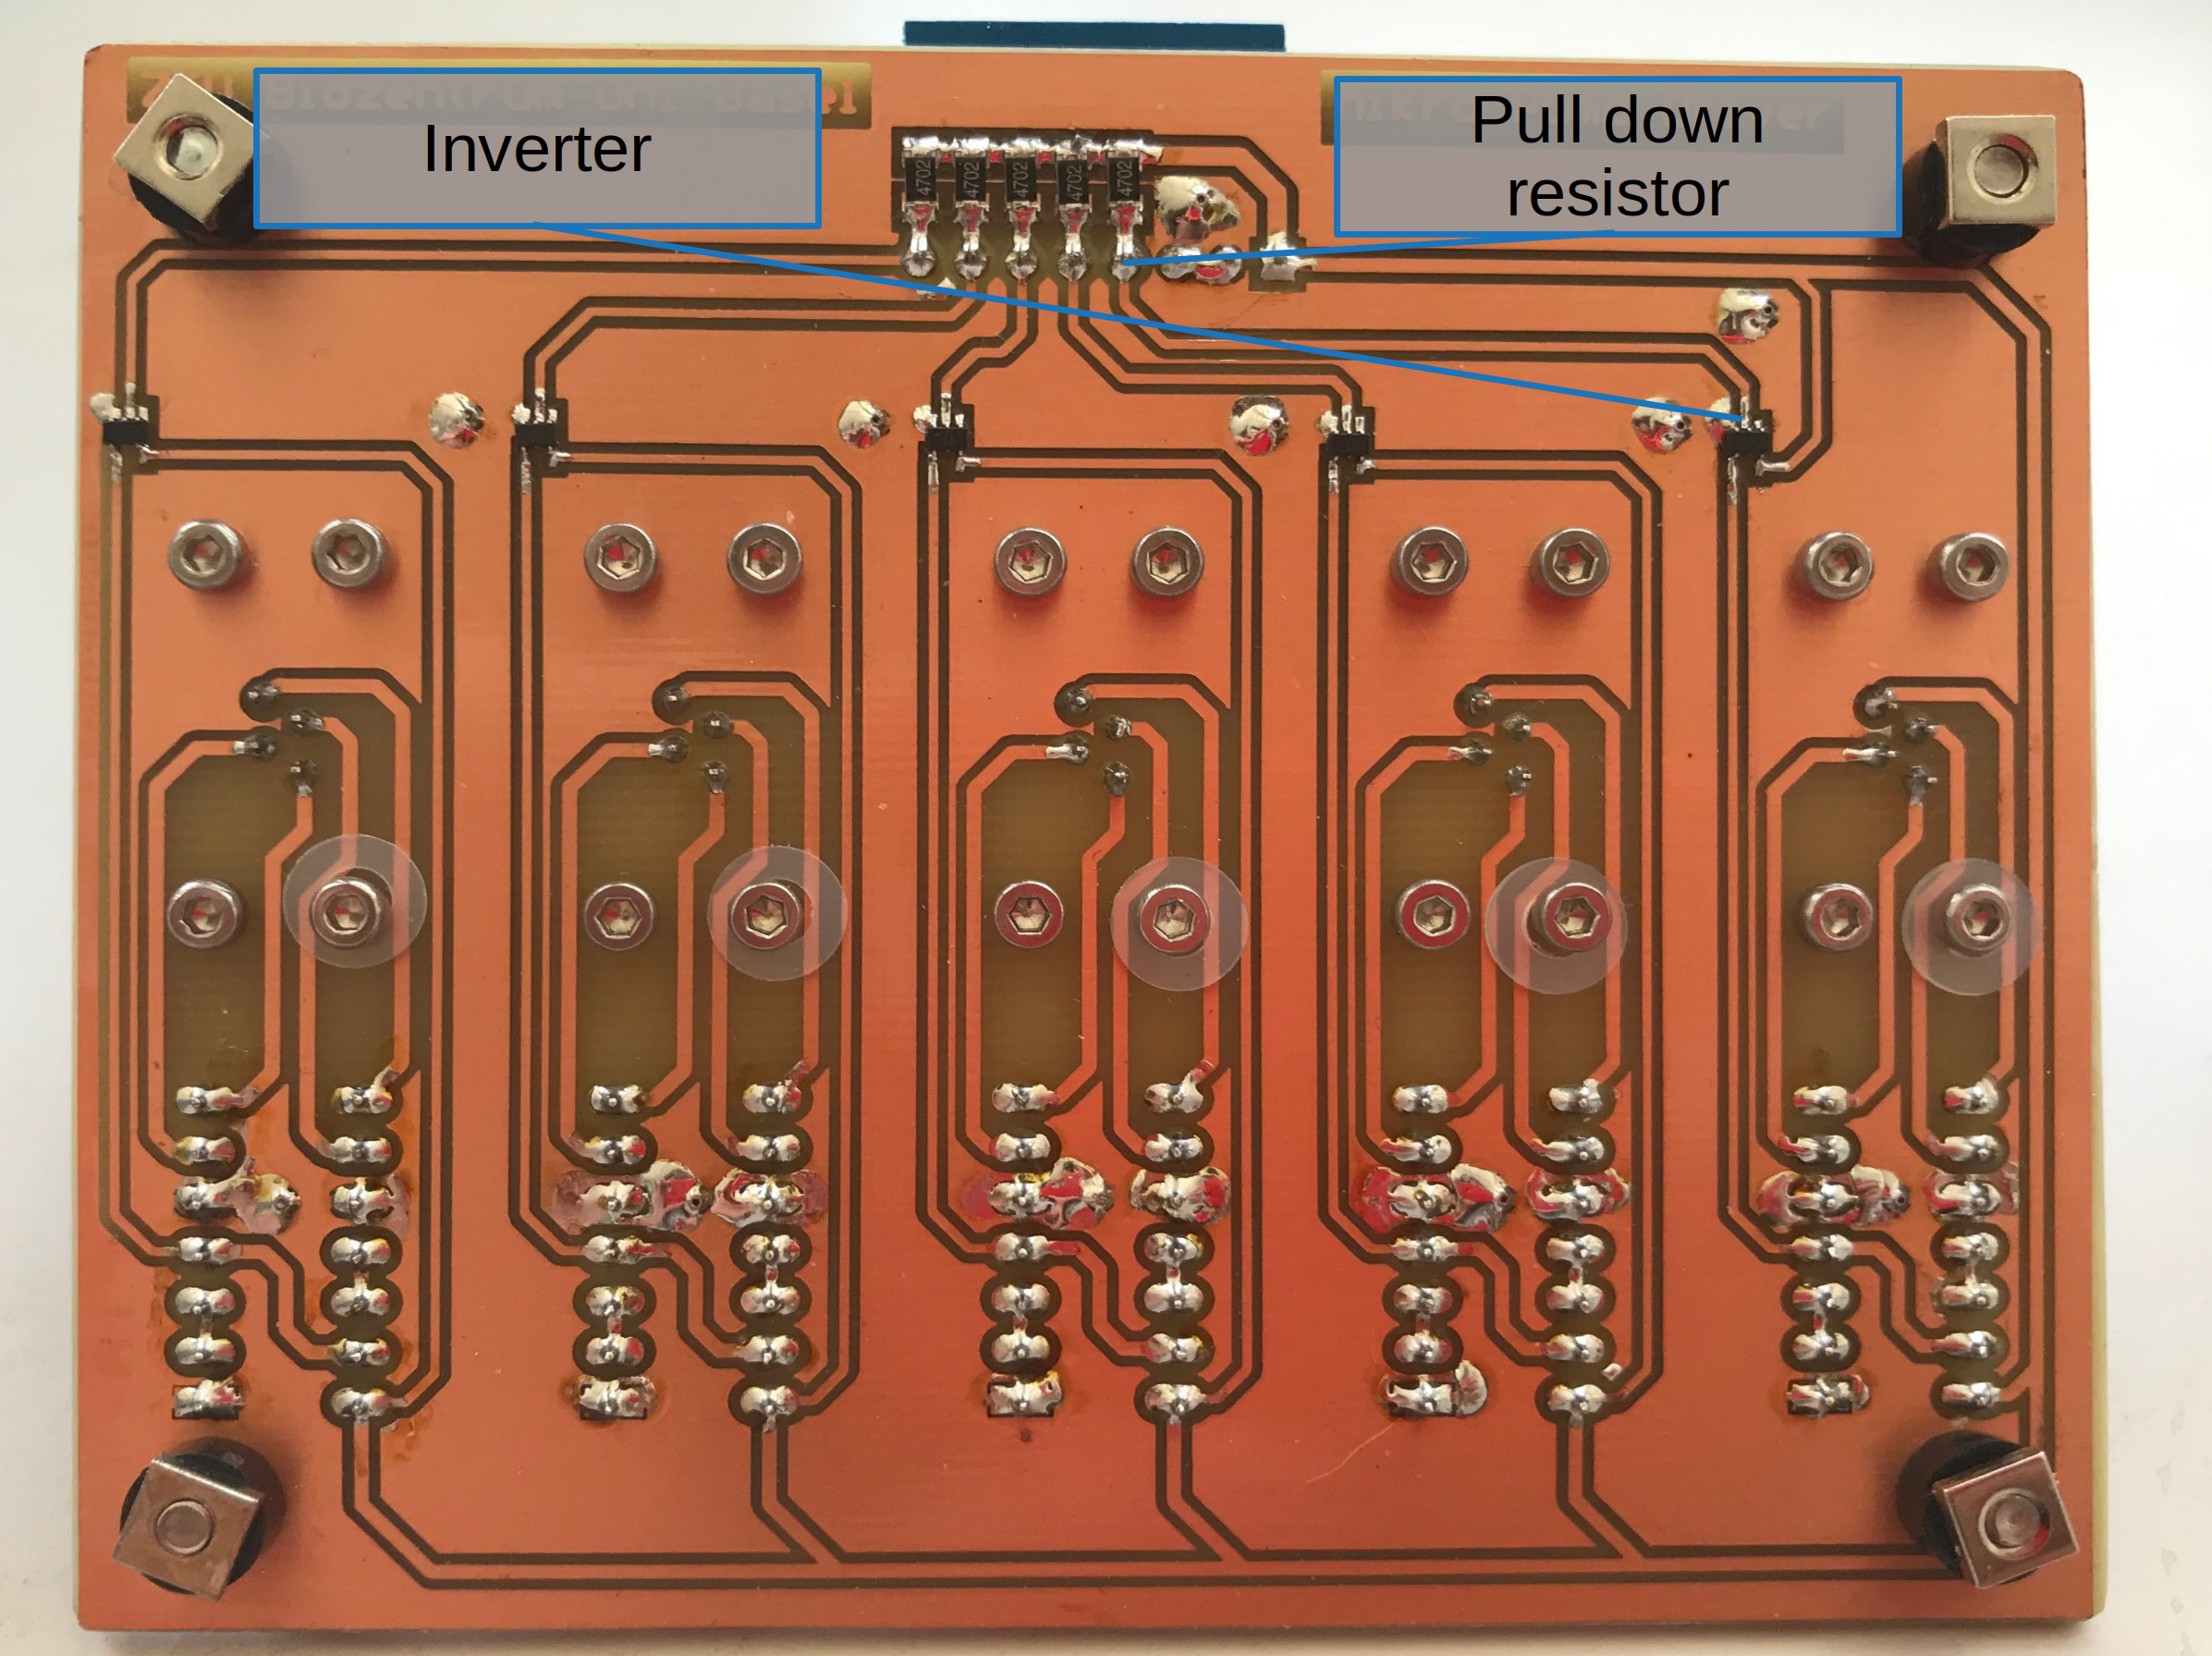
\includegraphics[width=0.4\textwidth]{board_below.png}
	\caption{Left: Principle of the piezo pumps. Top state: Piezo ceramic (purple) mounted on a membrane (blue) is relaxed. Left valve is open (orange), right valve  is closed, liquid enters. Right and bottom state: Voltage is applied to the piezo ceramic deforming the membrane resulting in a down stroke. Left valve is closed, right valve is open Liquid exits to the right. Voltage decreases again and the piezo ceramic enters its relaxed state again \cite{piezo_pumps}}. Middle: Top view of a circuit board with five pumps and five controllers. Right: Bottom view of a circuit board. 
	\label{figure:pumps}
\end{figure}
\begin{figure}
	\includegraphics[width=0.5\textwidth]{pump_blocks.JPG}
	\caption{Three pump boxes with five pumps and controllers stacked on top of each other. The outlets of the pumps were connected column by column and led to the vials.}
	\label{figure:tubing_setup}
\end{figure}
Every vial was connected to three injecting pumps. One pump was responsible for injecting media, one for injecting a low-concentrated antibiotic and one for injecting a high-concentrated antibiotic. Mixing of desired antibiotic concentrations was possible by controlling the run times of the pumps.
We chose mp6 pumps from microComponents because of their very compact build. The functional principle of the pumps is shown in the left Figure \ref{figure:pumps}. We achieved a steady flow rate of the pumps with the mp6-OEM controller from microComponents. On one circuit board five pumps with five mp6-OEM controllers were mounted which is shown in Figure \ref{figure:pumps}. Each mp6-OEM controller was connected to one pump, a 5 V power supply, a ground and a digital pin of the microcontroller which allowed computer controlling the run times of every pump. The circuit boards were mounted in a metal box and three of those boxes stacked on top of each other which is shown in Figure \ref{figure:tubing_setup}. By packing five pumps in a box and stacking three boxes on top of each other we were able to connect one row of vials to the whole range of antibiotic concentrations with one stack. Pumps of the lowest box were connected to media, pumps of the middle box to a low-concentrated antibiotic and the pumps of the top box to a high-concentrated antibiotic. We connected the outgoing tubes of the pumps from one stack column by column resulting in one outgoing tube per column as shown in Figure \ref{figure:tubing_setup}. Those tubes were led to the vials. This way we connected one vial with three pumps providing all concentrations of antibiotic and media with just one tube leading to the vial.\\
Every vial was also connected to a 16-channel peristaltic pump which removed volume exceeding the culture volume through the gray tube shown in the right Figure \ref{figure:morbidostat_setup}. 

\subsubsection{Computer controlling the pumps}
In order to control the run times of the pumps a pin of every mp6-OEM controller was connected with a digital pin of the microcontroller. If the pin of the mp6-OEM controller received a voltage of 5 V the pumps were off, if the pin was set to ground the pumps were on. \\
When we set the digital pins of the microcontroller to ground there was still a low current flowing, resulting in a small voltage. The mp6-OEM controllers reacted very sensitive to this small voltage leading to weird behavior of the pumps. We solved this by inserting a pull-down resistor between the digital pins of the microcontroller and the ground which is shown in Figure \ref{figure:pumps}. Additionally an inverter was connected in serial to the digital pins. To turn on a pump the digital pins of the microcontroller was set to 5 V. The inverter connected in serial set the signal at the pin of the mp6-OEM to ground and the pumps. Run time control was possible by setting the digital pins to 5 V for the desired time.
The 16-channel peristaltic pump was also computer controllable because the pump was also connected to a digital pin of the microcontroller.
\label{section:pumps}

\subsection{Controlling the morbidostat}
As a microcontroller we used an Arduino mega 2560 flashed with an arduino-script called \href{https://github.com/nahanoo/ESBL\_project/}{arduino\_morbidostat.ino}, which allowed us to change the state of digital pins or measuring voltages of analog pins. The microcontroller itself was controlled by a laptop where two python scripts were running. The python script \href{https://github.com/nahanoo/ESBL\_project/}{morbidostat\_experiment.py} decided which analog pins were measured and which digital pins were set to high for how long. Those tasks were grouped in cycles and repetitively executed. Additionally this script was responsible for storing ODs and injected antibiotic concentrations. We used a second python script called \href{https://github.com/nahanoo/ESBL\_project/}{arduino\_interface.py} to enable the communication between the laptop and the microcontroller. Commands for the microcontroller initialized by \href{https://github.com/nahanoo/ESBL\_project/}{morbidostat\_experiment.py} were encoded in a string by \href{https://github.com/nahanoo/ESBL\_project/}{arduino\_interface.py} which was transmitted to the microcontroller via a serial USB connection. The microcontroller interpreted the string and executed the encoded commands. \\
We implemented three modes for the morbidostat in \href{https://github.com/nahanoo/ESBL\_project/}{morbidostat\_experiment.py}. Those being the continuous mode which we used for continuous inhibition of the cultures, a growth rate mode where growth rates with no injections were recorded and a fixed OD mode where the OD of a culture was fixed to a certain OD by dilution with media. \\   

\subsubsection{Tasks of a continuous morbidostat cycle}
As for every mode the continuous mode consisted of several tasks grouped in one cycle. Shown in Figure \ref{figure:flowchart} as a first step the microcontroller measured the voltages of the analog pins connected to OD measuring units for a defined cycle time (typically being 10 minutes). Those voltages were constantly sent to the laptop where they were translated to ODs which were saved. After the cycle time the program fit a line to the OD measurements of a cycle for every vial. Using this fit the growth of every vial was calculated and stored. Additionally the measured ODs of a cycle where averaged and stored as well. Then a feedback algorithm calculated how much drug to inject into which vial. Shown in Figure \ref{figure:flowchart} the last step of a cycle was to translate the calculated antibiotic concentration into run times of the three pumps connected to a vial. The run times were sent to the microcontroller. The microcontroller turned on the pumps for the calculated time and after removing volume exceeding the culture volume with the peristaltic pump one cycle was finished. The injected volume was the same for every morbidostat experiment, which was controlled with the dilution factor.  \\
The commandflow of the growth rate mode was very similar just that the feedback function was not executed and therefore no fluids were injected into the vials. For the fixed OD mode another function instead of the feedback  calculated how much media to inject to keep the OD at a constant value. 

\begin{figure}
	\includegraphics[scale=0.25]{flowchart.png}
	\caption{Overview of one cycle from the continuous mode of the morbidostat.}
	\label{figure:flowchart}	
\end{figure}

\subsubsection{Feedback of the continuous mode} 
The feedback determined how strongly the cultures were inhibited with antibiotics. This feedback was based on the relative difference between the averaged ODs of the current cycle and the averaged ODs of a past cycle. We called the average ODs of a cycle final\_OD and the relative difference between two final\_ODs \textDelta OD. 
\begin{center}
	$\Delta OD = (final\_OD_{x_{cycles\_back}} - final\_OD_{current\_cycle})/x$ \quad (3.1) 
\end{center}
As shown in Figure \ref{figure:feedback} the feedback did several comparisons before calculating an appropriate dose of antibiotics. As a first step it checked if \textDelta OD was positive or negative. A negative \textDelta OD implied that the bacteria were dying. In order to prevent complete sterilization, media was injected in this case, effectively diluting the antibiotic concentration in the vial. \\
When \textDelta OD was positive the bacteria were growing. Antibiotics were only injected if the bacteria reached a certain OD called drug\_dilution\_threshold. Therefore, the next comparison as visible in Figure \ref{figure:feedback}, was whether or not the final\_OD was bigger or smaller than this threshold. If the final\_OD was smaller no fluids were injected.
However when final\_OD was bigger than the threshold, calculation of the appropriate dose was initialized.
The calculation itself was split up into two equations.
\begin{center}
	$increase\_vial\_conc = vial\_conc + mic\_fraction*mic$ \quad (I) \label{eq:plus}
\end{center}
\begin{center}	
	$increase\_vial\_conc = vial\_conc * c * \Delta OD/target\_OD$ \quad (II) \label{eq:mult}
\end{center}
Equation I, mainly important at the beginning of the morbidostat experiments, was used to approximate the MIC of the strains in the vials. This was done by simply adding a fraction of the MIC (mic\_fraction) to the current vial concentration (vial\_conc). After the MIC was reached this equation was ignored and from now on equation II determined the injected concentration. This equation multiplied the current drug concentration in the vials (vial\_ conc) by the \textDelta OD which resulted in how much the drug concentration in the vial was increased (increase\_ vial\_ conc).
The goal of the feedback was that a certain OD called target\_OD was approximated in every vial. In order to do so we divided the second equation by this target\_OD. Now if a small target\_OD was chosen the increased concentration was divided by a small value causing a higher injected concentration. If target\_OD was set to a high value the divided outcome was smaller. As a last step a constant (c) was introduced, which allowed to fine-tune the aggressiveness of the feedback.   

\begin{figure}
	\includegraphics[scale=0.13]{feedback.png}
	\caption{Schematic overview of decisions involved in the feedback.}
	\label{figure:feedback}
\end{figure}

\subsection{Hardware calibration}
\subsubsection{OD and pump calibration}
The OD measuring units were calibrated by measuring several cultures with a known OD.
An overnight culture with K12 XL1 blue E. coli was inoculated in 5 ml 9/10 $H_2O$ and 1/10 LB media (also referred to as diluted media). The next day the overnight culture was diluted 1/200 in 50 ml diluted media. After a few hours of day culturing following OD standards were prepared with 18 ml diluted media in the vials for the morbidostat: 0.01 0.021 0.042 0.107 0.192 0.278\\
Then every vial with a certain OD was placed in every vial holder. With the function calibrate\_OD from the \href{https://github.com/nahanoo/ESBL\_project/}{morbidostat\_experiment.py}, a voltage measurement was done for every OD standard and every OD measuring unit. The result of this function was a linear equation which translated the voltages to ODs. \\
\begin{figure}[H]
	\includegraphics[width=1\textwidth]{od_calibration.png}
	\caption{Calibration of OD measuring units, with the OD standards on the x-axis and the measured voltages on the y-axis. The line represents the calculated linear equation. The units of vial 5 and 15 were not working.}
\end{figure}
To determine the flow rate of the pumps the function calibrate\_pumps from the\href{https://github.com/nahanoo/ESBL\_project/}{morbidostat\_experiment.py} was executed. The weight of every empty vial had to be entered and the function turned on every specified pump for 100 seconds. Afterwards the weight of the vials was entered again and the function calculated the flow rate for the specified pumps. 
\label{section:OD_calibration}

\section{Experimentally evolving resistance with the morbidostat}
For evolving resistance with the morbidostat Beatrice Claudi from Dirk Bumanns group  produced three ESBL \textit{E. coli} strains, by assembling ESBL producing plasmids with Gibson cloning which were transformed into \textit{E. coli K-12} MG1655 \cite{bioz.com_bioz_nodate}. Working with ESBL \textit{E. coli K-12} MG1655 increased the safety of the handling, because \textit{E. coli K-12} MG1655 does not colonize the human intestine.\\
We cultured the ESBL \textit{E. coli} strains with the plasmid produced with gibson cloning with the morbidostat in the continuous mode leading to increased resistance to cefepime within a few days. To confirm emerged resistance the MIC of the strains was compared before and after culturing with the morbidostat. Samples taken while culturing with the morbidostat were Illumina and ONT sequenced. The resulting sequencing data was analyzed using the bioinformatic pipeline described in Section \ref{section:pipeline}.

\subsection{Gibson cloning}
\begin{figure}
	\includegraphics[width=0.45\textwidth]{pBC48_pSC101_PybaJ_mCherry-100_Neon-32_Map.png}
	\includegraphics[width=0.55\textwidth]{pEU22_p25_WT_CTX-M-1_134015_Map.png}
	\caption{Left: Vector used for Gibson cloning. Right: Resulting pEU22 plasmid. The insert, consisting of an ESBL gene and its regulatory sequence amplified with template DNA from patient isolates, replaced NeonGreen which allowed selection for clones with the insert.}
	\label{figure:vec}
\end{figure}
We extracted three ESBL gene sequences and their upstream sequence up to the previous gene (regulatory sequence) from two isolates of the isolate collection from the University Hospital of Basel (see Section \ref{section:sample_collection}). An identifier was created for every extracted gene with its regulatory sequence. The extracted sequences are shown in the supplementary in Section \ref{section:sequences}. Primers for PCR amplification were designed, based on the extracted sequences.
\begin{table}[H]
	\begin{tabular}{|llll|} \hline
		ID    & Product                & Source             	& Fragment size in bp \\ \hline
		pEU22 & \textbeta-lactamase CTX-M-1 & Patient 25 isolate 1 &	1614 \\ \hline
		pEU23 & \textbeta-lactamase OXA-1   & Patient 25 isolate 1 & 1789\\ \hline
		pEU26 & \textbeta-lactamase OXA-1   & Patient 33 isolate 1 & 1789\\ \hline
	\end{tabular}
	\label{table:plasmid}
	\caption{Designed insert for gibson cloning. The ESBL genes were amplified including its regulatory sequence. }
\end{table}
\begin{table}[H]
	\begin{tabularx}{\textwidth}{|ccL|}
		\hline
		ID    & Direction & Primer sequence                                                                        \\ \hline
		pEU22 & Reverse   & cgaagcagaaccccaTCATCCGAGAGCTTGCATGCC TGCAttacaaaccgtcggtgacgattttag             \\ \hline
		pEU22 & Forward   & GGCTCTTGTATCTATCAGTGAAGCATCAAGACTAAC AAATgcccacagaatgatgtcacgc                  \\ \hline
		pEU23 & Reverse   & cgaagcagaaccccaTCATCCGAGAGCTTGCATGCC TGCAttataaatttagtgtgtttagaatggtgatcgcatttt \\ \hline
		pEU23 & Forward   & GGCTCTTGTATCTATCAGTGAAGCATCAAGACTAAC AAATgtgatcccctgggcgaaatg                   \\ \hline
		pEU26 & Reverse   & cgaagcagaaccccaTCATCCGAGAGCTTGCATGCC TGCAttataaatttagtgtgtttagaatggtgatcgcatttt \\ \hline
		pEU26 & Forward   & GGCTCTTGTATCTATCAGTGAAGCATCAAGACTAAC AAATgtgatcccctgggcgaaatg                   \\ \hline
		Vector & Forward   & GGCTCTTGTATCTATCAGTGAAGCATCAAGACTAAC AAATgtgatcccctgggcgaaatg                   \\ \hline
		Vector & Reverse   & GGCTCTTGTATCTATCAGTGAAGCATCAAGACTAAC AAATgtgatcccctgggcgaaatg                   \\ \hline
	\end{tabularx}
	\label{table:primer}
	\caption{Primers used for the PCR amplification of the ESBL genes with their regulatory sequence and for controlling the insertion into the vector.}
\end{table}
The fragments were amplified using the primer sequences shown in Table \ref{table:primer} and the KOD-Hot-start-DNA plymerase with template DNA from the according isolate.
The vector shown in Figure \ref{figure:vec} was amplified by PCR as well using the iProof fidelity polymerase, its sequence is shown in the supplementary (see Section \ref{section:sequences}). All PCR reactions were loaded on a 1\% agarose gel. Since only bands with the expected lengths were present, the bands were cut out and purified using the NucleoSPin Gel and PCR Clean-up Kit. The DNA was eluted in 30 \textmu L nuclease-free water. 
The following Gibson reaction was prepared in order to insert the fragments into the vector:
\begin{table}[H]
	\begin{tabular}{|llllll|}
		\hline
		\multirow{2}{*}{ID}    & \multirow{2}{*}{Fragment} & \multirow{2}{*}{Conc. [ng/\textmu L]} & \multicolumn{3}{l|}{Volume [\textmu L]}           \\
		&                           &                                       & DNA  & GIBSON MIX         & $H_2O$                  \\ \hline
		\multirow{2}{*}{pEU22} & Insert                    & 268                                   & 0.22 & \multirow{2}{*}{5} & \multirow{2}{*}{2.75} \\
		& Vector                    & 25.66                                 & 2.03 &                    &                       \\ \hline
		\multirow{2}{*}{pEU23} & Insert                    & 342.9                                 & 0.19 & \multirow{2}{*}{5} & \multirow{2}{*}{2.78} \\
		& Vector                    & 25.66                                 & 2.03 &                    &                       \\ \hline
		\multirow{2}{*}{pEU26} & Insert                     & 285.2                                 & 0.22 & \multirow{2}{*}{5} & \multirow{2}{*}{2.74} \\
		& Vector                    & 25.66                                 & 2.03 &                    &                       \\ \hline
	\end{tabular}
	\caption{Gibson reaction with the inserts, the vector and the GIBSON mix.}
\end{table}
The reactions were incubated for 20 min at 50 \degree C. From the reactions 2 \textmu L was added to 100 \textmu L electrocompetent cells of the strain \textit{E. coli K-12 MG1655}. The mixture was electroporated with a Bio-Rad electroporator, pelleted and resuspended in 1 mL super optimal broth. The cells were shaken for 2 hours at 180 rpm and 37 \degree C. The electroporated strains were plated on LB plates containing kanamycin  and grown over night. Because our vector includes a kanamycin resistance gene, all colonies which grew on the plates had the plasmid.  Additionally, the vector had two genes coding for fluorescence proteins, mCherry (red) and NeonGreen (green). As seen in Figure \ref{figure:vec} the insert replaced the gene coding for NeonGreen. Therefore the Gibson reaction was only successful for clones which were not green. Only red clones were picked and grown over night in LB containing kanamycin. Based on those cultures the clones were checked with a PCR. As a forward primer 'TCTCAATGGTTCGTTCTCATGG' was used, as a reverse primer 'GGAACAGTACGAACGCGCCGA' was used. The PCR control showed positive results and the strains were stocked in LB containing 20\% glycerol.
The ID created for the plasmids was adopted for the strains. 

\subsection{Culturing ESBL \textit{E. coli} strains with the morbidostat}
Before culturing with the morbidostat, we determined the MIC of the ESBL \textit{E. coli} strains and sterilized the device.

\subsubsection{MIC determination}
We inoculated 5 ml of MHB media with the ESBL \textit{E. coli} strains and cultured the suspension over night at 37 \degree C. The next day a 1/100 dilution in 20 ml MHB was prepared for every suspension and cultured for a few hours at 37 \degree C. The growth of the day cultures was constantly monitored by measuring the OD. When the OD of the day culture was 0.08, a 1/100 dilution of every day culture was prepared. \\
We added 100 \textmu L of MHB to every well of a 96 well plate. Except for the last column of the plate, we added 100 \textmu L of the diluted day culture to every well. 100 \textmu L of a cefepime solution with a concentration of 2.048 mg/mL was added to the first column of the plate. Starting from the first column a 1:1 dilution series was prepared with the the first seven columns. We incubated the plates for 16 hours at 37 \degree \space on a shaker. To get an idea how many cells were used for the MIC determination $10^{-3}$ and $10^{-5}$ dilutions of the 1/100 diluted cell cultures were plated on LB plates.\\
After 16 hours the OD of every well was measured using a plate reader. The smallest concentration which inhibited the growth was determined as the MIC. 
\label{section:mic_determination}

\subsubsection{Sterilization of the morbidostat}
We sterilized the morbidostat using two different disinfectants in order to prevent biofilm formation and contamination of our vials.
Bottles, vials, tubing and luer connections were autoclaved. Sterile vials were connected to the tubes and the computer controllable pumps were connected to 1 L of 3 \% citric acid stored in a sterile bottle with sterile tubing. All the tubing going to the vials was flushed with the disinfectant over one hour. The waste pump was turned on leading to disinfection of the tubes connected to the sterile waste bottle. After that the tubing was flushed with 1 L of sterile water. We repeated this procedure but this time using 3 \% of bleach as disinfectant.
\label{section:sterilization}

\subsubsection{Culturing with the morbidostat}
We ran two morbidostat experiments with the ID 01 and 02 with the ESBL \textit{E. coli} strains and \textit{E.coli K-12} MG1655 as a control. For every experiment we prepared over night cultures of the ESBL \textit{E. coli} strains in 3 ml diluted media with 3 \textmu L kanamycin. \textit{E. coli K-12} MG1655 was cultured over night in 3 mL diluted media. The over night cultures were diluted 200 fold the next day and cultured for a few hours. From those cultures, 200 \textmu L were transferred into sterile vials containing 18 mL diluted media. We prepared two different antibiotic concentrations which were connected to the pumps. We prepared a concentration of 9 \textmu g/ml cefepime in 1 L diluted media as a low-concentrated antibiotic solution. For the high-concentrated solution we prepared a cefepime concentration of 21 \textmu g/mL in 1 L diluted media. The morbidostat experiments were initialized with a target\_OD of 0.12, and a dilution factor of 0.91. Every ESBL \textit{E. coli} strain was cultured at least three times with the continuous mode. Additionally we cultured every ESBL \textit{E. coli} strain with the fixed\_OD mode. The temperature inside the hypoxi-station was set to 37 \degree C. The $O_2$ level was fixed to 10 \% and $CO_2$ fixed to 5 \%. \\
As resistance evolved the antibiotic concentrations of the bottles were changed. We checked which concentration was necessary to strongly inhibit the cultures. New cefepime concentrations which were 3 fold and 7 fold higher than the newly determined inhibiting concentration were prepared and connected. We changed the antibiotic concentrations of the bottles approximately every third day. If the suspension in the vials was extremely milk caused by dead cells we transferred 200 \textmu L of the suspension to a new sterile vial containing 18 ml diluted media.  \\
During both experiments we took daily samples by opening the vial in the hypoxi-station and transferring 1 mL to an eppendorf tube. The collected samples were centrifuged at 13'000 rpm for 10 minutes and resuspended in 200 \textmu L LB containing 20 \% glycerol. Those suspensions were frozen at -80 \degree C.\\

\subsection{Analysis of the morbidostat samples}
\subsubsection{Illumina and Nanopore sequencing}
We handed the stocks of the cloned ESBL \textit{E. coli} strains and K-12 MG1655 to our collaborators of the University Hospital of Basel where they were sequenced on a MiSeq-Illumina system (see Section \ref{section:illumina}).
Furthermore, we handed them the stocks for Illumina sequencing of the last sample day of every vial form the 01 experiment. 
From the 02 experiment we selected the stocks from vial 3,4,5,7 and 8 from the third sample day and the stocks from every vial of the last sample day for Illumina sequencing. Every stock that we handed over for Illumina sequencing was stroked out. 
We sequenced the ESBL \textit{E. coli} stocks and K-12 MG1655 with ONT. For DNA extraction we inoculated 3 mL LB containing 1 \% kanamycin with the ESBL \textit{E. coli} stocks. K-12 MG1655 was inoculated in 3 mL LB. The suspensions were cultured over night. The DNA of the resulting over night cultures was extracted following the protocol of the DNeasy Blood \& Tissue Kit (50). The extracted DNA was sequenced with a MinION as described in Section \ref{section:nanopore_sequenicng}. 

\subsubsection{Contamination analysis}
On the plates where we stroked out every stock that we handed over for Illumina sequencing we saw colonies which had a different shape than \textit{E. coli}. Therefore, we had the suspicion that some stocks were contaminated. Because we had Illumina sequencing data for every stock we could identify the contamination by blasting a few reads \cite{madden_blast_2003}. This revealed that the contamination was \textit{Bacillus cereus}. To identify which samples were contaminated, all the Illumina short-reads from every stock  were mapped to a \textit{Bacillus cereus} reference genome obtained from NCBI \cite{noauthor_bacillus_nodate} and the ESBL \textit{E. coli} reference genome produced with hybrid-assembling.

\subsubsection{Identifying mutations in morbidostat samples}
The sample series from the morbidostat experiments were analyzed following the bioinformatic pipeline described in Section \ref{section:pipeline}. 

\chapter{Results}
\section{Analyzing ESBL E. coli isolates from patients of the University hospital Basel}
\subsection{Selection of samples suitable for our analysis}
We could only analyze sample series of a patient consisting of multiple samples. Furthermore the MICs of samples in a series had to change significantly. As a last criteria all the ESBL \textit{E. coli} strains of a series had to be the same.

The phylogenetic tree of all samples is shown in Figure \ref{figure:panX}. This tree revealed that many patients were infected with different ESBL \textit{E. coli} strains over time. This was visible in the tree when samples of one patient mapped on different branches. Interestingly some samples from different patients mapped on the same branch which suggests that those patients were infected from the same outbreak. The selected patients and the MICs of their ESBL \textit{E. coli} samples is shown in Table \ref{table:samples}.

\begin{figure}
	\includegraphics[scale=0.2]{181205_panXtree_overview.png}
	\caption{Phylogenic tree built for every ESBL \textit{E. coli} sample}
	\label{figure:panX}
\end{figure}


\begin{table}[]
	\begin{tabularx}{\textwidth}{|cccLL|}
		\hline
		Patient                   & Sample                   & Sample date                     & MIC cefepim {[}\textmu g/ml{]} & MIC ceftazidime {[}\textmu g/ml{]} \\ \hline
		\rowcolor[HTML]{FFCE93} 
		{\color[HTML]{000000} 12} & {\color[HTML]{000000} 0} & {\color[HTML]{000000} 09/09/14} & {\color[HTML]{000000} 4}                      & {\color[HTML]{000000} 0.75}                       \\
		& 1                        & 05/12/14                        & 12                                            & 2                                                 \\ \hline
		\rowcolor[HTML]{FFCE93} 
		16                        & 0                        & 22/06/12                        & 8                                             & 2                                                 \\
		& 1                        & 18/07/13                        & 48                                            & 8                                                 \\
		& 2                        & 01/11/13                        & 32                                            & 12                                                \\ \hline
		\rowcolor[HTML]{FFCE93} 
		24                        & 0                        & 02/05/11                        & 4                                             & 1.5                                               \\
		& 1                        & 08/15/11                        & 16                                            & 1.5                                               \\
		& 2                        & 11/28/11                        & 3                                             & 1                                                 \\ \hline
		25                        & 0                        & 15/04/11                        & 64                                            & 192                                               \\
		\rowcolor[HTML]{FFCE93} 
		& 1                        & 22/08/11                        & 6                                             & 6                                                 \\ \hline
		33                        & 0                        & 26/09/14                        & 6                                             & 6                                                 \\
		\rowcolor[HTML]{FFCE93} 
		& 1                        & 29/01/15                        & 1                                             & 1.5                                               \\ \hline
	\end{tabularx}
	\caption{Selected patients and the MIC of cefepim and ceftazidime for their ESBL \textit{E. coli} samples. Samples stained in orange were chosen as reference genomes.}
	\label{table:samples}
\end{table}
\subsection{Identification of mutations}
For patient 12,16 and 24 we chose sample 0, for patient 25 and 33 we chose sample 1 for building a reference genome. The selected samples are stained orange in \ref{table:samples}.
The output of the ONT sequencing for the reference genomes and in how many contigs they were hybrid-assembled is shown in Table \ref{table:reference_genomes} 

\begin{table}[]
	\begin{tabularx}{\textwidth}{|ccLLL|}
		\hline
		Patient & Sample & Gigabases sequneced with ONT & Hybrid-assemlied in n contigs & ONT coverage \\ \hline
		12      & 0      & 0.39                         & 6                             & 73           \\ \hline
		16      & 0      & 1.11                         & 3                             & 207          \\ \hline
		24      & 0      & 1.81                         & 17                            & 336          \\ \hline
		25      & 1      & 1.82                         & 12                            & 338          \\ \hline
		33      & 1      & 1.24                         & 6                             & 231          \\ \hline
	\end{tabularx}
	\caption{Output of ONT sequencing for the reference genomes and in how many contigs the genomes were hybrid-assemblied}
	\label{table:reference_genomes}
\end{table} 
\subsection{Identified mutations for the selected sample series}
\subsubsection{Patient 12}
Our bioinformatial pipeline revealed two mutations for patient 12 which are shown in \ref{table:patient12}. For those mutations our pipeline didn't find any annotation. 
\begin{table}[H]
	\begin{tabularx}{\linewidth}{|cccLL|}
		\hline
		\#SNP & Contig & Position & \multicolumn{2}{l|}{Nucleotide in Sample:} \\
		&        &          & 0         & \multicolumn{1}{l|}{1}    \\ \hline
		1 & 0 & 880249  & C & A \\ \hline
		2 & 0 & 4256761 & A & T \\ \hline
	\end{tabularx}
	\caption{SNPs of sample series of patient 12}
	\label{table:patient12}
\end{table} 
\subsubsection{Patient 16}
In Table \ref{table:patietn16} we show the identified mutatios for the sample series of patient 16. We identified 21 mutations, seven of those where deletions and the rest were SNPs. Our pipeline found annotation for seven mutations. Six mutations affected genes and one mutation affected a promoter. The affected genes are shown in Table \ref{table:pat16annot} and the affected promoter in Table \ref{table:pat16_prom}. This promoter annotation was obtained from the EcoCyc promoter sequences. 
\begin{table}[H]
	\begin{tabularx}{\linewidth}{|cccLLL|}
		\hline
		\#SNP & Contig & Position & \multicolumn{3}{l|}{Nucleotide in Sample:} \\
		&        &          & 0     & 1     & \multicolumn{1}{l|}{2}    \\ \hline
		1     & 0      & 109928   & C     & A     & \multicolumn{1}{l|}{C}    \\ \hline
		2     & 0      & 1895312  & A     & C     & \multicolumn{1}{l|}{A}    \\ \hline
		3     & 0      & 2101128  & G     & -     & \multicolumn{1}{l|}{-}    \\ 
		&        & 2101129  & C     & -     & \multicolumn{1}{l|}{-}    \\ 
		&        & 2101130  & A     & -     & \multicolumn{1}{l|}{-}    \\ \hline
		4     & 0      & 2375277  & C     & T     & \multicolumn{1}{l|}{C}    \\ \hline
		5     & 0      & 3797984  & A     & G     & \multicolumn{1}{l|}{A}    \\ \hline
		6     & 0      & 4200032  & T     & C     & \multicolumn{1}{l|}{T}    \\ \hline
		7     & 0      & 4353560  & G     & C     & \multicolumn{1}{l|}{G}    \\ \hline
		8     & 0      & 5112127  & G     & T     & \multicolumn{1}{l|}{G}    \\ \hline
		9     & 0      & 55597    & A     & G     & \multicolumn{1}{l|}{G}    \\ \hline
		10    & 0      & 922702   & G     & A     & \multicolumn{1}{l|}{G}    \\ \hline
		11    & 0      & 1133762  & C     & T     & \multicolumn{1}{l|}{T}    \\ \hline
		12    & 0      & 1549518  & T     & G     & \multicolumn{1}{l|}{G}    \\ \hline
		13    & 0      & 2016331  & A     & C     & \multicolumn{1}{l|}{A}    \\ \hline
		14    & 0      & 2101129  & C     & -     & \multicolumn{1}{l|}{-}    \\ 
		&        & 2101130  & A     & -     & \multicolumn{1}{l|}{-}    \\ \hline
		15    & 0      & 3920934  & A     & G     & \multicolumn{1}{l|}{A}    \\ \hline
		16    & 0      & 4333944  & C     & T     & \multicolumn{1}{l|}{T}    \\ \hline
		17    & 0      & 4459680  & C     & -     & \multicolumn{1}{l|}{C}    \\ 
		&        & 4459681  & C     & -     & \multicolumn{1}{l|}{C}    \\ \hline
		18    & 0      & 4459684  & G     & -     & \multicolumn{1}{l|}{G}    \\ 
		&        & 4459685  & A     & -     & \multicolumn{1}{l|}{A}    \\ 
		&        & 4459686  & A     & -     & \multicolumn{1}{l|}{A}    \\ 
		&        & 4459687  & G     & -     & \multicolumn{1}{l|}{G}    \\ 
		&        & 4459688  & A     & -     & \multicolumn{1}{l|}{A}    \\ 
		&        & 4459689  & G     & -     & \multicolumn{1}{l|}{G}    \\ \hline
		19    & 0      & 4459692  & A     & -     & \multicolumn{1}{l|}{A}    \\ 
		&        & 4459693  & G     & -     & \multicolumn{1}{l|}{G}    \\ \hline
		20    & 0      & 4459695  & G     & -     & \multicolumn{1}{l|}{G}    \\ \hline
		21    & 0      & 4459697  & T     & -     & \multicolumn{1}{l|}{T}    \\ \hline
	\end{tabularx}
	\caption{Mutations of the sample series of patient 16.}
	\label{table:patietn16}
\end{table}
\begin{table}[H]
	\begin{tabularx}{\linewidth}{|ccLLccc|}
		\hline
		\#SNP & Gene          & Product                                  & Type and position in gene      & \multicolumn{3}{l|}{Amino acid in Sample:} \\
		&               &                                          &                        & 0   & 1               & 2               \\ \hline
		1     & \textit{ortT} & Orphan toxin OrtT                        & Missense, 44           & P   & T               & P               \\ \hline
		2     & \textit{scrY} & Sucrose Porin                            & Missense, 104          & L   & V               & L               \\ \hline
		3     & \textit{cpdA} & Phosphodiesterase CpdA                   & In-frame deletion, 162 & L   & -   & -   \\ \hline
		4     & \textit{rpoB} & DNA-directed RNA polymerase subunit beta & Missense, 113          & V   & I               & V               \\ \hline
		5     & \textit{ftsQ} & Cell division protein FtsQ               & Missense, 207          & K   & R               & K               \\ \hline
		4     & \textit{recR} & Recombination protein RecR               & Missense, 40           & M   & T               & M               \\ \hline
		5     & \textit{hcxA} & Hydoxycarboxylate dehydrogenase A        & Missense, 332          & R   & G               & R               \\ \hline
		6     & \textit{ribA} & GRP cyclohydrolase-2                     & Missense, 68           & F   & L               & L               \\ \hline
	\end{tabularx}
	\caption{Annotation for identified Mutations, type and how they affected the peptide for patient 16.}
	\label{table:pat16annot}  
\end{table}
\begin{table}[H]
	\begin{tabular}{|lll|}
		\hline
		\#SNP & Transcription unit & Next upstream gene \\ \hline
		16    & fes-ybdZ-entF-fepE & \textit{fepA}      \\ \hline
	\end{tabular}
	\caption{Identified promoter affected by a mutation}
	\label{table:pat16_prom}
\end{table}
The mutation at position 80 in the fepA promoter is shown in the Alignment \ref{figure:alignment}. The mutation was found in the binding site of the \textsigma 70 transcription factor.  
\begin{texshade}{pat16fepa.aln}
	\showruler{1}{top}
		\feature{bottom}{1}{24..29}{fill:-}{-35}
	\feature{bottom}{1}{48..53}{fill:-}{-10}
	\feature{top}{1}{60..60}{fill:$\downarrow$}{Start of $\sigma$70 binding site}
	\hideconsensus
	\showcaption{This alignment shows the SNP in the fepA promotor. Positions marked with dashed lines are the recognition sites for $\sigma$70 factor.}
	\label{figure:alignment}
\end{texshade}
\subsubsection{Patient 24}
Identified mutations for the sample series of patient 24 are show in Table \ref{table:pat24} and the affected genes in Table \ref{table:pat24_ann}.
\begin{table}[H]
	\begin{tabularx}{\linewidth}{|cccLLL|}
		\hline
		\#SNP & Contig & Position & \multicolumn{3}{l|}{Nucleotide in Sample:} \\
			&        &          & 0     & 1     & \multicolumn{1}{l|}{2}    \\ \hline
	1     & 0      & 50032    & G            & A            & G            \\ \hline
	2     & 0      & 418564   & C            & T            & C            \\ \hline
	3     & 0      & 2048961  & A            & C            & C            \\ \hline
	4     & 0      & 2319554  & T            & A            & A            \\ \hline
	5     & 0      & 3444478  & T            & C            & T            \\ \hline
	6     & 0      & 4063226  & G            & T            & T            \\ \hline
	\end{tabularx}
	\caption{Identified mutations for patient 24}
	\label{table:pat24}
\end{table}

\begin{table}[H]
	\begin{tabularx}{\linewidth}{|ccLLccc|}
		\hline
		\#SNP & Gene          & Product                                  & Type and position in gene      & \multicolumn{3}{l|}{Amino acid in Sample:} \\
		&               &                                          &                        & 0   & 1               & 2               \\ \hline
		1     & \textit{atl}     & DNA base-flipping protein                                  & Missense, 87      & V           & M           & V           \\ \hline
		2     & \textit{imm\_2}  & Colicin-E7 immunity protein                                & Missense, 69      & K           & E           & K           \\ \hline
		3     & \textit{lldR\_2} & Lactate Dehydrogenase regulatory protein & Missense, 44      & I           & S           & S           \\ \hline
		4     & \textit{dctM\_2} & TRAP transporter large permease protein                                                        & Missense, 112     & T           & S           & S           \\ \hline
		5     & \textit{dltA}    & D-alanine--D-alanyl carrier protein ligase subunit 1           & Missense, 692     & E           & G           & E           \\ \hline
		6     & \textit{fnr}     & Fumarate and nitrate reduction regulatory protein          & Missense, 31      & C           & F & F  \\ \hline    
	\end{tabularx}
	\caption{Annotation for identified Mutations, type and how they affected the peptide for patient 24.}
	\label{table:pat24_ann}
\end{table}

\subsubsection{Patient 25}
For the sample series of patient 25 six mutations were identified, one of them is a deletion of 12 nucleotides causing a frame-shift mutation in the peptide. The mutations are shown in Table \ref{table:pat25} and their annotations in Table \ref{table:pat25_ann}.

\begin{table}[H]
	\begin{tabularx}{\linewidth}{|cccLL|}
		\hline
		\#SNP & Contig & Position & \multicolumn{2}{l|}{Nucleotide in Sample:} \\
		&        &          & 0         & \multicolumn{1}{l|}{1}    \\ \hline
	1 & 0 & 396325   & G & A \\ \hline
	2 & 0 & 396846  & G & A \\ \hline
	3 & 0 & 1996537 & - & C \\ 
	&   & 1996538 & - & C \\ 
	&   & 1996539 & - & G \\ 
	&   & 1996540 & - & T \\ 
	&   & 1996541 & - & A \\ 
	&   & 1996542 & - & C \\ 
	&   & 1996543 & - & C \\ 
	&   & 1996544 & - & A \\ 
	&   & 1996545 & - & G \\ 
	&   & 1996546 & - & C \\ 
	&   & 1996547 & - & T \\ 
	&   & 1996548 & - & G \\ \hline
	4 & 0 & 3743644 & A & G \\ \hline
	5 & 0 & 4785433 & G & A \\ \hline
	6 & 0 & 4785439 & G & A \\ \hline
	\end{tabularx}
	\caption{Identified mutations for patient 25}
	\label{table:pat25}
\end{table} 

\begin{table}[H]
	\begin{tabularx}{\linewidth}{|ccLLcc|}
		\hline
	\#SNP & Gene          & Product                                 & Type and position & \multicolumn{2}{l|}{Amino acid Sample:} \\
	&               &                                         &                   & 0                  & 1                  \\ \hline
	1     & \textit{ompR} & Transcriptional regulatory protein OmpR & Missense, 146     & R                  & H                  \\ \hline
	2     & \textit{envZ} & Osmolarity sensor protein EnvZ          & Missense, 84      & G                  & E                  \\ \hline
	3     & \textit{rfbD} & dTDP-4-dehydrorhamnose reductase        & \multicolumn{3}{l|}{Frameshift deletion, 148-295}            \\ \hline
	\end{tabularx}
	\caption{Annotation for identified Mutations, type and how they affected the peptide for patient 25.}
	\label{table:pat25_ann}
\end{table}

\subsubsection{Patient 33}
Only three mutations were found for the sample series of patient 33, they are shown in Table \ref{table:pat33} with their annotation in Table \ref{table:pat33_ann}.
\begin{table}[H]
	\begin{tabularx}{\linewidth}{|cccLL|}
		\hline
		\#SNP & Contig & Position & \multicolumn{2}{l|}{Nucleotide in Sample:} \\
		&        &          & 0         & \multicolumn{1}{l|}{1}    \\ \hline
		1 & 0 & 4008745 & A & T \\ \hline
		2 & 0 & 4675092 & T & A \\ \hline
		3 & 0 & 1996537 & A & C \\ \hline
	\end{tabularx}
	\caption{Identified mutations for patient 25}
	\label{table:pat33}
\end{table} 
\begin{table}[H]
	\begin{tabularx}{\linewidth}{|ccLLcc|}
		\hline
		\#SNP & Gene          & Product                           & Type and position & \multicolumn{2}{l|}{Amino acid Sample:} \\
		&               &                                   &                   & 0                  & 1                  \\ \hline
		1     & \textit{cydD} & ATP-binding/permease protein CydD & Missense, 368     & Q                  & L                  \\ \hline
		2     & \textit{vnfA} & Nitrogen fixation protein VnfA    & Missense, 169     & N                  & I                  \\ \hline
	\end{tabularx}
	\caption{Annotation for identified Mutations, type and how they affected the peptide for patient 16.}
	\label{table:pat33_ann}
\end{table}
\subsection{Copynumbers of ESBL genes}
Next to the reference genomes we also hybrid-assemblied and annotated the other samples of the selected sample series. This allowed us to see, if the copy numbers of ESBL genes increased while resistance evolved. Which ESBL genes where present on a plasmid or chromosomally in which sample is shown in Figure \ref{figure:esbl_genes}. For four out of five patients the copy number remained very similar. Sometimes the ESBL gene was integrated in the chromosome or an ESBL gene was replaced by a different ESBL gene. Only the sample series of patient 33 showed an increase of ESBL genes while resistance evolved. Sample 0 of patient 33 has 9 copies of CTX-M-1 while sample 1 only had one. 
\begin{figure}[H]
	\includegraphics[width=.25\textwidth]{pat12s0.png}
	\includegraphics[width=.25\textwidth]{pat12s1.png}	
	
	\includegraphics[width=.25\textwidth]{pat16s0.png}
	\includegraphics[width=.25\textwidth]{pat16s1.png}
	\includegraphics[width=.25\textwidth]{pat16s2.png}
	
	\includegraphics[width=.25\textwidth]{pat24s0.png}
	\includegraphics[width=.25\textwidth]{pat24s1.png}
	\includegraphics[width=.25\textwidth]{pat24s2.png}
	
	\includegraphics[width=.25\textwidth]{pat25s0.png}\hfill	
	\includegraphics[width=.25\textwidth]{pat25s1.png}\hfill
	\includegraphics[width=.25\textwidth]{pat33s0.png}\hfill
	\includegraphics[width=.25\textwidth]{pat33s1.png}\hfill
	
	\caption{Copy numbers of ESBL genes. A-B: Copy numbers for patient 12 stayed the same. C-E: One CTX-M-1 was integrated in the genome for sample 1. F-H: Sample 2 lost CTX-M-97 but picked up one copy of TEM. I-J: Copy numbers for patient 25 stayed the same. K-L: Sample 1 has 8 more copies of CTX-M-1.}
	\label{figure:esbl_genes}
\end{figure}
Studying the short-reads of sample 0 mapped to the reference genome from sample 1 revealed that the coverage for sample 0 was very high for a region of 17 kilo base-pairs (kbp). This increased coverage, the genes located within this region and the GC-content is shown in Figure \ref{figure:coverage}. The gene coding for CTX-M-1 is within this 17 kbp region. This confirms that the copy number of the gene coding for CTX-M-1 is much higher in sample 0.

\begin{figure}[H]
	\includegraphics[scale=0.3]{coverage_pat33.png}
	\caption{Upper figure: Annotation of the whole plasmid. Middle figure: Coverage of the illumina sequencing data from sample 0 (resistant sample) and sample 1 (susceptible sample). Buttom figure: GC content.}
	\label{figure:coverage}
\end{figure}
\newpage
\newpage
\section{Morbidostat experiments}
\subsection{Contamination analysis}
\begin{table}[H]
	\begin{tabularx}{\linewidth}{|LLLLL|}
		\hline
		Stocked strain    & Total reads & Reads mapped to \textit{Bacillus cereus} & Reads mapped to \textit{E. coli} & \% of reads mapped to \textit{Bacillus cereus} \\ \hline
		pEU22\_CTX & 3810442     & 16496                                                     & 3803789                                           & 0.43                                                            \\ \hline
		pEU23\_OXA & 4329090     & 18499                                                     & 4322708                                           & 0.43                                                            \\ \hline
		pEU26\_OXA & 4040571     & 17629                                                     & 4036167                                           & 0.44                                                            \\ \hline
		K-12 MG 1655      & 4939319     & 21902                                                     & 4931214                                           & 0.44                                                            \\ \hline
	\end{tabularx}
	\caption{Illumina short-reads from every stock were mapped to a \textit{Bacillus cereus} genome from NCBI \cite{noauthor_bacillus_nodate} and the \textit{E.coli} reference genome produced with  hybrid-assembling.}
	\label{table:bacillus_reads}
\end{table}
\begin{figure}
\includegraphics[width=0.8\textwidth]{bacillus_reads.png}
\caption{Alignment of short reads from pEU23\_OXA to the \textit{Bacillus cereus}. The reads map with a few SNPs which are colored. The reads also don't overlap.}
\label{figure:bacillus_reads}
\end{figure}
As visible in Table \ref{table:bacillus_reads} around 0.44 \% of all Illumina short-reads map to \textit{Bacillus cereus}. In Figure \ref{figure:bacillus_reads} one region of an alignment of the Illumina short-reads to the \textit{Bacillus cereus} genome is shown. We could see that those reads only map to very certain regions of the genome without overlapping and with a variation of a few bases. Because the reads are not overlapping and they don't map with an identity of 100 \% the stocks were not contaminated. Also the hybrid-assembly of the reference genome did not show any contigs with \textit{Bacillus cereus} sequences.
This means that around 0.44 \% of the plasmid-stocks map to conserved regions of the \textit{Bacillus cereus} genome. Therefore we expect a similar outcome for the samples from the morbidostat which were not contaminated. 

The outcome of mapping the Illumina shor-reads from the morbidostat samples to the \textit{Bacillus cereus} reference genome and the \textit{E. coli} reference genome of the sample is shown in Table \ref{table:bacillus_reads_samples}.
12 samples were not contaminated and 9 were pretty heavily contaminated.
\begin{table}[H]
	\begin{tabularx}{\linewidth}{|LccLLLL|}
		\hline
		Experiment & Vial & Sample & Total reads & Reads mapped to \textit{Bacillus cereus} & Reads mapped to \textit{E. coli} & \% of reads mapped to \textit{Bacillus cereus} \\ \hline
		01         & 1    & 1      & 6490750     & 4967611                         & 272289                  & 76.53                                \\ \hline
		01         & 2    & 1      & 7601839     & 6001106                         & 418578                  & 78.94                                \\ \hline
		01         & 3    & 1      & 2940556     & 13976                           & 2934902                 & 0.48                                 \\ \hline
		01         & 4    & 1      & 8167777     & 6150829                         & 281584                  & 75.31                                \\ \hline
		01         & 5    & 1      & 5606842     & 4089104                         & 178462                  & 72.93                                \\ \hline
		01         & 9    & 1      & 5636939     & 4466280                         & 268813                  & 79.23                                \\ \hline
		01         & 10   & 1      & 4935808     & 22368                           & 4928816                 & 0.45                                 \\ \hline
		02         & 1    & 1      & 6152378     & 26815                           & 6143228                 & 0.44                                 \\ \hline
		02         & 2    & 1      & 6926506     & 5180940                         & 291927                  & 74.80                                \\ \hline
		02         & 3    & 1      & 5142535     & 24909                           & 5136761                 & 0.48                                 \\ \hline
		02         & 3    & 2      & 6196309     & 4694898                         & 279679                  & 75.77                                \\ \hline
		02         & 4    & 1      & 4923087     & 22342                           & 4915639                 & 0.45                                 \\ \hline
		02         & 4    & 2      & 4589212     & 20628                           & 4582915                 & 0.45                                 \\ \hline
		02         & 5    & 1      & 4298753     & 17870                           & 4292083                 & 0.42                                 \\ \hline
		02         & 5    & 2      & 5189054     & 22772                           & 5181923                 & 0.44                                 \\ \hline
		02         & 7    & 1      & 5167596     & 22583                           & 5159028                 & 0.44                                 \\ \hline
		02         & 7    & 2      & 4976635     & 3015316                         & 107767                  & 60.59                                \\ \hline
		02         & 8    & 1      & 4356280     & 19067                           & 4350598                 & 0.44                                 \\ \hline
		02         & 8    & 2      & 4186125     & 18526                           & 4181356                 & 0.44                                 \\ \hline
		02         & 9    & 1      & 4182681     & 18487                           & 4176477                 & 0.44                                 \\ \hline
		02         & 10   & 1      & 3809536     & 2576863                         & 136340                  & 67.64                                \\ \hline
	\end{tabularx}
	\caption{Illumina short-reads from every morbidostat sample mapped to to a \textit{Bacillus cereus} from NCBI \cite{noauthor_bacillus_nodate} and the \textit{E.coli} reference genome produced with  hybrid-assembling.}
	\label{table:bacillus_reads_samples}
\end{table}
The identified SNPs and affected proteins are shown for every vial with samples which were not contaminated.
\subsection{Experiment 01}
\subsubsection{Vial 3}
No SNPs were found for this vial.
\subsubsection{Vial 10}
\begin{table}[H]
	\begin{tabularx}{\linewidth}{|cccLL|}
		\hline
		\#SNP & Contig & Position & \multicolumn{2}{l|}{Nucleotide in Sample:} \\
		&        &          & 0         & \multicolumn{1}{l|}{1}    \\ \hline
		1 & 0 & 3403729 & G & C \\ \hline
	\end{tabularx}
\end{table} 
\begin{table}[H]
	\begin{tabularx}{\linewidth}{|ccLLcc|}
		\hline
		\#SNP & Gene          & Product                           & Type and position & \multicolumn{2}{l|}{Amino acid Sample:} \\
		&               &                                   &                   & 0                  & 1                  \\ \hline
	1 & \textit{tomB\_1} & Hha toxicity modulator TomB & Silent, 43 & I & V \\ \hline
	
	\end{tabularx}
\end{table}
\subsection{Experiment 02}
\subsubsection{Vial 1}
No SNPs were found for this vial.
\subsubsection{Vial 3}
\begin{table}[H]
	\begin{tabularx}{\linewidth}{|cccLL|}
		\hline
		\#SNP & Contig & Position & \multicolumn{2}{l|}{Nucleotide in Sample:} \\
		&        &          & 0         & \multicolumn{1}{l|}{1}    \\ \hline
		1 & 1 & 4290 & G & T \\ \hline
	\end{tabularx}
\end{table} 
The identified SNP is affecting the cloned plasmid. More coming soon. 
\subsubsection{Vial 4}
\begin{table}[H]
	\begin{tabularx}{\linewidth}{|cccLLL|}
		\hline
		\#SNP & Contig & Position & \multicolumn{3}{l|}{Nucleotide in Sample:} \\
		&        &          & 0     & 1     & \multicolumn{1}{l|}{2}    \\ \hline
		1 & 1 & 2526   & T & T & A \\ \hline
		2 & 0 & 347328 & C & C & T \\ \hline
	\end{tabularx}
\end{table}

\begin{table}[H]
	\begin{tabularx}{\linewidth}{|ccLLccc|}
		\hline
		\#SNP & Gene          & Product                                  & Type and position in gene      & \multicolumn{3}{l|}{Amino acid in Sample:} \\
		&               &                                          &                        & 0   & 1               & 2               \\ \hline
		1 & \textit{bla}  & Beta-lactamase CTX-M-1                  & Missense, 289 & V & V & D \\ \hline
		2 & \textit{ompR} & Transcriptional regulatory protein OmpR & Nonsense, 67  & R & R & * \\ \hline
	\end{tabularx}
\end{table}
\subsubsection{Vial 5}
\begin{table}[H]
	\begin{tabularx}{\linewidth}{|cccLLL|}
		\hline
		\#SNP & Contig & Position & \multicolumn{3}{l|}{Nucleotide in Sample:} \\
		&        &          & 0     & 1     & \multicolumn{1}{l|}{2}    \\ \hline
		1 & 0 & 1570984 & C & C & T \\ \hline
		2 & 0 & 668881  & A & T & A \\ \hline
		3 & 0 & 2898640 & G & G & - \\ \hline
	\end{tabularx}
\end{table}

\begin{table}[H]
	\begin{tabularx}{\linewidth}{|ccLLccc|}
		\hline
		\#SNP & Gene          & Product                                  & Type and position in gene      & \multicolumn{3}{l|}{Amino acid in Sample:} \\
		&               &                                          &                        & 0   & 1               & 2               \\ \hline
		1 & \textit{ompC\_1} & Outer membrane protein C         & Silent, 8              & L & L & L \\ \hline
		2 & \textit{rpoD}    & RNA polymerase sigma factor RpoD & Missense, 594             & L & Q & L \\ \hline
		3 & \textit{ompF}    & Outer membrane protein F         & Frameshift, 319 & G & G & A \\ \hline
	\end{tabularx}
\end{table}
\subsubsection{Vial 8}
No SNPs were found for this vial.
\subsubsection{Vial 9}
\begin{table}[H]
	\begin{tabularx}{\linewidth}{|cccLL|}
		\hline
		\#SNP & Contig & Position & \multicolumn{2}{l|}{Nucleotide in Sample:} \\
		&        &          & 0         & \multicolumn{1}{l|}{1}    \\ \hline
		1 & 0 & 3076603 & A & T \\ \hline
	\end{tabularx}
\end{table} 
\begin{table}[H]
	\begin{tabularx}{\linewidth}{|ccLLcc|}
		\hline
		\#SNP & Gene          & Product                           & Type and position & \multicolumn{2}{l|}{Amino acid Sample:} \\
		&               &                                   &                   & 0                  & 1                  \\ \hline
1 & \textit{iscR} & HTH-type transcriptional regulator IscR & Missense, 56 & C & S \\ \hline

		
	\end{tabularx}
\end{table}


\chapter{Discussion}
In this thesis the evolution of cefepime resistance in ESBL \textit{E. coli} was studied. A bioinformatic pipeline was established, which we used to identify SNPs in the genome while resistance to cefepime evolved in ESBL \textit{E. coli}. This pipeline was applied to next generation sequencing data of ESBL isolates sampled from patients at the University Hospital of Basel. Furthermore, we assembled a morbidostat which we used to experimentally evolve cefepime resistance in ESBL \textit{E. coli}. Samples taken from the morbidostat were analyzed with the established bioinformatic pipeline as well. 
Technical and experimental challenges are discussed in the following as well as the potential relevance of the identified SNPs and their annotation for cefepime resistance.

\section{Technical and experimental challenges with the morbidostat}
\subsection{Hardware issues}
We faced problems with the computer controllable pumps that we used for injecting antibiotics and media. The controllers and the piezo pumps were very sensitive to small currents flowing through the digital pins of the microcontroller. This caused malfunctions of the pumps. We were able to fix this issue by connecting pull-down resistors to the digital pins of the microcontroller and the ground. Furthermore, we connected inverters in serial to the digital pins, which increased the reliability of the pumps.\\
We observed in the morbidostat experiment 01 that stirring created air cones which affected the OD measurements. This is why we had to reduce the stirring to a minimum. Generally, strong stirring could be beneficial because it would guarantee equal antibiotic concentrations in the vials. Stirring could be increased if the OD measuring units would be lowered. \\
We used vials with a polytetrafluoroethylene (Teflon) insert with holes through which we inserted plastic tubes acting as vial inserts. Even though the holes for the plastic tubes were drilled as small as possible, the plastic tubes started to loosen up over time, which we tried to fix by adding silicone. Because of the physical properties of polytetrafluoroethylene silicone did not stick and the plastic tubes could not be sealed properly. Therefore, some vials may have not been completely sealed, potentially increasing the risk of contamination. Furthermore, the chosen vial design was not ideal for sampling, because we had to unscrew the lid of the vials in the hypoxi-station, which increased the risk of introducing contaminations.
\subsection{Software issues}
Our microcontroller could only execute one task after the other. This means that we had to ensure that the python script was sending the commands one after another, instead of sending multiple commands at once. Therefore, we had to thread the commands.  Even though we threaded the commands, we encountered a problem with the microcontroller, caused by receiving multiple commands at once. The OD measurements potentially interfered with changing the state of the digital pins and the microcontroller crashed. The pumps did not turn off and the vials were overflowing. Therefore, we added a reset function which recognized when the microcontroller crashes and automatically hard resets the microcontroller.   

\subsection{\textit{Bacillus cereus} contamination of the morbidostat experiments}
The majority of our vials were contaminated with \textit{Bacillus cereus}. Since all the stocked strains which we used for starting morbidostat experiments were not contaminated, the contamination must have entered the system during the experiment. Alternatively, sterilization was not successful. For sterilizing we used 1 L of 3\% citric acid and 1 L of 3\% bleach. Both solutions were pumped through all the tubing over one hour. Additionally, every piece of hardware in contact with fluids, except the pumps, were autoclaved. \textit{Bacillus cereus} is a gram-positive, endospore-forming bacteria \cite{bintsis_foodborne_2017}. It is possible that \textit{Bacillus cereus} endospores overcame the sterilization protocol. A study reported that after exposing \textit{Bacillus cereus} endospores to 10\% bleach for 15 minutes, they were still able to produce colonies \cite{robertson_effect_2018}. Alternatively, the \textit{Bacillus cereus} contamination entered the system while taking samples or exchanging the media and drug bottles. As already discussed, the design of the vials was not ideal and contaminations could have entered the device through gaps in the vial inserts. It is also possible that some tube connections were not completely sealed allowing contaminations to enter the device.  \\
Cefepime is supposed to be especially active against gram-positive bacteria \cite{sykes_chapter_2014}. Therefore, it is generally surprising, that \textit{Bacillus cereus} survived culturing with high doses of cefepime. \textit{Bacillus cereus} might have taken up the ESBL plasmid from the ESBL \textit{E. coli} strains by natural competence, which decreased their susceptibility. Possibly, \textit{Bacillus cereus} was killed by the high cefepime concentration, but the antibiotic pressure induced the formation of endospores. For sequencing we inoculated LB containing kanamycin with the sample stocks and cultured them overnight. During overnight culturing the endospores might could have switched to the vegetative cycle, causing the contamination in the stocks to be passed for sequencing.

\section{Bioinformatic challenges}
Generally, we identified more mutations in patient isolates than in morbidostat samples. For example the isolates of patient 16 revealed 21 SNPs. One source for this observation  could be that some patients got reinfected with different ESBL \textit{E. coli} strains, even though we tried to ensure strain identity by phylogenetic analysis. Potentially, the phylogenetic tree was not fully resolved and some strains, assumed to be identical, but were actually different. The environment during morbidostat experiments can be fully controlled, because we cultured in the hypoxi-station. The nutrient concentration remained the same, because we cultured with diluted LB media throughout the whole experiment. Therefore, the antibiotic pressure was the main stress causing evolution. On the other hand, in patient isolates the strains had to adapt to many more environmental factors which could further explain why more SNPs were identified in patient isolates. Likely, many patients were treated with other drugs than antibiotics as well, which could also cause evolution of the ESBL \textit{E. coli} strains. \\
For the isolate series of patient 25 and patient 33 the resistance decreased over the sampling period, which is the opposite compared to the other patient isolate series and the sample series from the morbidostat. For those two resistance did not evolve over the sampling period. Therefore, we defined the most recent sample with the lowest resistance level as reference and identified SNPs in the earliest samples with high resistance levels. We still consider the identified SNPs as relevant, because it is still likely that they can be associated with the corresponding high resistance level. We would have preferred to analyze more isolate series where resistance evolved over the sampling period, but we were restricted by the isolate collection at hand. \\
The bioinformatic pipeline for identifying SNPs proved to be solid. \textit{De novo} whole-genome assembling with ONT and Illumina sequencing data using the assembler Unicycler resulted in accurate whole-genomes, positively affected by the high coverage that we achieved with ONT sequencing \cite{wick_unicycler:_2017}. The rest of the pipeline consisted of established bioinformatic steps such as mapping Illumina reads to reference genomes and identifying SNPs with coverage and base frequency filtering. The weakness of the bioinformatic pipeline was the annotation of the SNPs. For some SNPs no annotation was found by prokka, the tool we used for annotating our reference genome, but blasting of the affected sequences revealed annotations for some additional SNPs \cite{seemann_prokka:_2014}.
However, we only presented annotations found by prokka \cite{seemann_prokka:_2014}.

\section{Culturing with the morbidostat}
The assembled morbidostat and the developed feedback algorithm worked very well. The designed OD measuring units proved to be rather sensitive, with the ability to detect ODs starting from 0.01. After optimizing the control of the injecting pumps, they showed to be very reliable and their compact design allowed easy handling of the morbidostat within the space-limited hypoxi-station.
The feedback reacted very well to the cultures by diluting with media when the bacteria were dying or by increasing antibiotic concentration if they grew very fast. The developed feedback algorithm might have allowed resistance to evolve faster than expected. Dösselmann \textit{et al.} reported that they cultured \textit{Pseudomonas aeruginosa} with a morbidostat and colistin for 20 days to achieve a 100-fold increase in MIC \cite{doselmann_rapid_2017}. We cultured ESBL \textit{E. coli} for only 5 days with our morbidostat and cefepime to achieve a similar increase of the MIC. Since the organism and the antibiotic are not identical, it is difficult to compare how fast resistance evolved. The performed morbidostat experiments proved that our version of the morbidostat is very capable to evolve resistance over a short period of time. 

\section{Potential resistance mechanisms considering mutated operons}mo
The identified SNPs in ESBL \textit{E. coli} patient isolates and morbidostat samples mainly suggested two targets, which could play an important role in cefepime resistance. One of the targets were porins, in particular the outer membrane protein F (OmpF), the outer membrane protein C (OmpC)  and their shared regulatory system. The other target was the RNA polymerase and the sigma factor. 
\subsection{SNPs in porin operons}
There are two major outer membrane proteins \textit{E. coli}, OmpF and OmpC \cite{rampersaud_ompr_1994}. Both are porins in the outer membrane through which cephalosporins pass \cite{masi_structure_2013}. A lack of those porins likely heavily reduces the cefepime uptake. Becerio A \textit{et. al} reported that two cefepime resistant ESBL \textit{E. coli} isolates lacked the OmpC and OmpF porins showing the importance of those porins for cefepime resistance \cite{beceiro_false_2011}.  Depending on the osmolarity of the environment \textit{ompF} or \textit{ompC} is preferably expressed. This is regulated by an osmolarity sensor protein EnvZ. EnvZ is a transmembrane sensor which detects the osmotic pressure and phosphorylates the transcriptional regulatory protein OmpR depending on the detected osmolarity \cite{rampersaud_ompr_1994}. At low osmolarity, EnvZ modulates low levels of phosphorylated OmpR, at high osmolarity EnvZ mediates high levels of phosphorylated OmpR \cite{rampersaud_ompr_1994}. OmpR is a DNA-binding protein which binds specific regions depending on its phosphorylation status and it is essential for the expression of \textit{ompC} and \textit{ompF} \cite{rampersaud_ompr_1994}. Phosphorylated OmpR binds to the promoter of \textit{ompC}, if OmpR is unphosphorylated it binds to the promoter of \textit{ompF} \cite{rampersaud_ompr_1994}. Therefore, phosphorylated OmpR increases the expression of the \textit{ompC} gene while repressing the expression of the \textit{ompF} gene \cite{rampersaud_ompr_1994}. On the other hand, OmpR which is not phosphorylated increases the expression of \textit{ompF} and reduces the expression of \textit{ompC}. \\
We found several SNPs in genes of the expressions system of \textit{ompF} and \textit{ompC} in patient isolates and morbidostat samples. One SNP in \textit{envZ} in a patient isolate, in \textit{ompR} one SNP was found in a patient isolate as well as in a morbidostat sample. In the patient isolate the SNP caused a missense mutation in OmpR, whereas in the morbidostat samples the SNP caused a nonsense mutation in OmpR. A mutated OmpR is potentially not able to bind to the the promoters of \textit{ompC} and \textit{ompF}, which could heavily reduce the expression of both outer membrane proteins. This seems especially plausible for the mutated OmpR in the morbidostat sample, because the nonsense mutation heavily impacts the functionality of the protein. The mutated \textit{envZ} found in a patient isolate potentially also affects the expression levels of \textit{ompC} and \textit{ompF}. In \textit{ompC} and \textit{ompF} itself we also found SNPs in morbidostat samples. While \textit{ompC} was affected by a SNP causing a silent mutation in OmpC, the mutation in \textit{ompF} caused a missense mutation in OmpF. The missense mutation in OmpF could cause a change of the structure of the porin, which potentially affects the permeability of the outer membrane for cefepime.\\
We found another SNP in the promoter of \textit{fepA}. FepA is a gated porin transporting unspecific hydrophilic substances \cite{liu_permeability_1993}. The mutation in the promoter potentially repressed the expression of \textit{fepA} which may further decrease the membrane permeability for cefepime. 

\subsection{SNPs in the transcription machinery operon}
SNPs were identified targeting the transcription machinery in patient isolates and morbidostat samples. In one patient isolate we found that a mutation in \textit{rpoB} coding for the DNA-directed RNA polymerase subunit \textbeta. In a morbidostat sample we found a SNP targeting \textit{rpoD} coding for the RNA polymerase sigma factor. This strongly suggests that some process in the RNA transcription is affecting the cefepime susceptibility. In a preprint Samantha Palace \textit{et al.} reported that they found a SNP in \textit{rpoB} in three ceftriaxone (a third-generation cephalosporin) resistant \textit{Neisseria gonorrhoeae} isolates \cite{palace_rna_2019}. They were able to recreate resistance by integrating the mutation in a ceftriaxone susceptible \textit{Neisseria gonorrhoeae} strain, proving the importance of the mutation for ceftriaxone resistance \cite{palace_rna_2019}. The mutation in \textit{rpoB} that they identified in not the same as the one that we found. They also reported a mutation in \textit{rpoD} in two \textit{Neisseria gonorrhoeae} isolates and were able to recreate resistance for this mutation \cite{palace_rna_2019}. Interestingly, it is not understood yet, how mutations in RpoB or RpoD are impacting cephalosporin resistance. 
\subsection{SNPs affecting other operons}
We also identified SNPs in genes for which the evidence was less clear that they potentially impact cefepime susceptibility. For example, one SNP was found in \textit{ortT}. OrtT is a toxin causing membrane damage resulting in reduced growth and increased persistence during stress related to amino acid and DNA synthesis \cite{islam_orphan_2015}.  Cells in the persistent state are generally thought to be more tolerant to antibiotics \cite{islam_orphan_2015}. While it is difficult to hypothesize why a mutated OrtT was beneficial for the strain, it makes sense that the persistent state is beneficial if antibiotic pressure is applied.  \\
One SNP affected the ESBL gene coding for \textbeta-lactamase CTX-M-1 in a morbidostat sample. This caused a missense mutation in the ESBL. The resulting variant is not know in the literature, therefore, it is not possible to estimate whether it is potentially degrading \textbeta-lactams more effectively compared to the wild-type. 
\section{Conclusion}
We studied cefepime resistance evolution in ESBL \textit{E. coli} patient isolates sampled at the University Hospital of Basel and assembled a morbidostat, which we used to experimentally evolve cefepime resistance in ESBL \textit{E. coli} strains. The assembled morbidostat showed great functionality, increasing the MIC over 100-fold compared to the MIC at the beginning. The bioinformatic analysis of the patient isolates and samples from morbidostat experiments revealed several SNPs in the genomes of ESBL \textit{E. coli} which evolved resistance. Interestingly, some SNPs were found in the same gene in patient isolates and morbidostat samples, strongly suggesting their relevance for cefepime resistance. Two systems were targeted independently by SNPs. One system were the porins, in particular the porins OmpD, OmpF and their regulatory proteins OmpR and EnvZ. The SNPs found in the porin operons could imply, that the expression level of the porins is reduced, potentially increasing the impermeability of the outer membrane for cefepime. For the other system which was targeted by SNPs, the DNA-directed RNA polymerase subunit \textbeta \space and its RNA polymerase sigma factor, the potential connection to cefepime resistance is unknown. Since the system was targeted by SNPs in patient isolates and morbidostat samples, it is still likely that the identified genotypes are affecting cefepime susceptibility. \\
With our genomic study of cefepime resistance evolution we could identified new genotypes which may impact cefepime susceptibility. Our findings support the relevance of other resistance mechanisms than cefepime degradation by \textbeta-lactamases which was the main focus of cefepime resistance investigations so far.  
\section{Outlook}
Our goal for future morbidostat experiments is to eliminate contaminations and repeat the resistance evolution experiments with the ESBL \textit{E. coli} strains that we used for this thesis. In order to eliminate the contaminations we will take several additional precautions. We will change the design of the vials and replace the polytetrafluoroethylene inserts with the plastic tubes by septa and syringes. This will guarantee sealed vials and will also improve sampling, because the septa allow sampling with a syringe without opening the vial, reducing the risk of contaminations. We also realized that the injecting pumps were autoclavable, which was the only piece of hardware in contact with fluids, which we had not autoclaved before the morbidostat experiments. In the future we will autoclave the pumps which eliminates further potential sources of contaminations. When we will repeat the morbidostat experiments without contaminations we expect to identify SNPs in the same genes confirming our current findings. \\
We will also try to extend our patient isolate collection sampled at the University of Basel and we will analyze the additional isolates with the existing bioinformatic pipeline.  \\
To finally confirm the importance of the identified SNPs, we could try to insert some identified mutations in cefepime susceptible \textit{E. coli} strains and check if the created genotypes show changed cefepime susceptibility. If so, this would suggest that the identified SNP is associated with cefepime resistance evolution. Once the morbidostat experiments have been repeated, we could also use the morbidostat for studying resistance evolution of other bacteria and antibiotics.
\chapter{Supplementary}
\section{Manual for starting experiments with morbidostat}
\label{section:manual}




\chapter{References}
\printbibliography
\includepdf[pages=-]{/home/ericulrich/masterarbeit/LaTeX_thesis/Declaration/Images/dec.pdf}
\end{document}
